\documentclass[9pt,conference]{IEEEtran}
\IEEEoverridecommandlockouts
\usepackage[top=1.18cm,bottom=1.18cm,left=1.20cm,right=1.20cm,columnsep=0.40cm]{geometry}
\usepackage[utf8]{inputenc}
\usepackage[T1]{fontenc}
\usepackage[brazil]{babel}
\usepackage{amsmath,amssymb,amsfonts}
\usepackage{graphicx}
\usepackage{textcomp}
\usepackage{xcolor}
\usepackage{booktabs}
\usepackage{multirow}
\usepackage{microtype}
\usepackage{url}
\usepackage{hyperref}
\usepackage{enumitem}

\setlist[enumerate]{leftmargin=*, noitemsep, topsep=2pt, partopsep=0pt, parsep=0pt}
\setlist[itemize]{leftmargin=*, noitemsep, topsep=2pt, partopsep=0pt, parsep=0pt}

\definecolor{unbblue}{RGB}{0,51,102}
\definecolor{unbgreen}{RGB}{0,102,51}
\definecolor{codebg}{RGB}{247,249,252}

\hypersetup{
    colorlinks=true,
    linkcolor=unbblue,
    citecolor=unbblue,
    urlcolor=unbblue
}

\setlength{\textfloatsep}{3.5pt plus 1pt minus 1pt}
\setlength{\floatsep}{3.5pt plus 1pt minus 1pt}
\setlength{\intextsep}{3.5pt plus 1pt minus 1pt}
\setlength{\dbltextfloatsep}{4pt plus 1pt minus 1pt}
\setlength{\dblfloatsep}{4pt plus 1pt minus 1pt}
\setlength{\abovecaptionskip}{2pt}
\setlength{\belowcaptionskip}{2pt}
\setlength{\abovedisplayskip}{3.5pt plus 1pt minus 1pt}
\setlength{\belowdisplayskip}{3.5pt plus 1pt minus 1pt}
\renewcommand{\arraystretch}{1.02}
\setlength{\tabcolsep}{3.2pt}

\begin{document}

\title{Controle Din\^{a}mico de ``Overthinking'' em Modelos de Linguagem via Parada Precoce Calibrada por Entropia em Cadeias de Pensamento (\textit{Chain-of-Thought})}

\author{\IEEEauthorblockN{Kelvin Rafael Paulino Buss}
\IEEEauthorblockA{\textit{Departamento de Ci\^{e}ncia da Computa\c{c}\~{a}o (CIC) -- P\'{o}s-Gradua\c{c}\~{a}o em Inform\'{a}tica (PPGI)} \\
\textit{Programa de P\'{o}s-Gradua\c{c}\~{a}o em Sistemas Mecatr\^{o}nicos (PPMEC)} \\
\textit{Universidade de Bras\'{i}lia (UnB)} -- Bras\'{i}lia, DF, Brasil \\
kelvin.buss@aluno.unb.br \\
Reposit\'{o}rio GitHub: \url{https://github.com/kelvinbuss/ProjetoFinalRNAP_UnB2026}}
\and
\IEEEauthorblockN{Prof. Dr. D\'{i}bio Leandro Borges}
\IEEEauthorblockA{\textit{Departamento de Ci\^{e}ncia da Computa\c{c}\~{a}o (CIC)} \\
\textit{Instituto de Ci\^{e}ncias Exatas (IE)} \\
\textit{Universidade de Bras\'{i}lia (UnB)} -- Bras\'{i}lia, DF, Brasil \\
dibio@unb.br}
}

\maketitle

\begin{abstract}
O escalonamento de computa\c{c}\~{a}o em tempo de teste (\textit{Test-Time Compute}) por meio de Cadeias de Pensamento (\textit{Chain-of-Thought} -- CoT) e vota\c{c}\~{a}o por \textit{Self-Consistency} (SC) consolidou-se como o paradigma dominante para amplificar a capacidade de racioc\'{i}nio matem\'{a}tico e simb\'{o}lico em Grandes Modelos de Linguagem (LLMs). Todavia, investiga\c{c}\~{o}es recentes apresentadas no ICLR 2026 demonstram que, em modelos de linguagem compactos (\textit{Small Language Models} -- SLMs, de 1,5B a 3B de par\^{a}metros), o prolongamento irrestrito das cadeias de racioc\'{i}nio n\~{a}o produz ganhos monot\^{o}nicos: a acur\'{a}cia segue uma curva em ``U invertido'' em fun\c{c}\~{a}o do comprimento $L$ da cadeia (\textit{overthinking}) (WU et al., 2026), sofrendo degrada\c{c}\~{a}o por sobrecorre\c{c}\~{a}o (\textit{over-correction}) (HAO et al., 2026) e dilui\c{c}\~{a}o de aten\c{c}\~{a}o em contextos extensos (FENG et al., 2026). Embora m\'{e}todos de escalonamento calibrado como o CaTS (HUANG et al., 2026) reduzam o n\'{u}mero de trajet\'{o}rias amostradas ($N$), eles ignoram a dimens\~{a}o intratrilha ($L$) e sofrem severa descalibra\c{c}\~{a}o quando trilhas longas inflam artificialmente a confian\c{c}a de tokens repetitivos. Este artigo prop\~{o}e o \textbf{LC-SC (\textit{Length-Calibrated Self-Consistency})}, um algoritmo de decodifica\c{c}\~{a}o online que controla conjuntamente a matriz de or\c{c}amento computacional $N \times L$ durante a infer\^{e}ncia. O LC-SC monitora em tempo real a entropia de Shannon token a token ($H_t$) para acionar tr\^{e}s mecanismos sin\'{e}rgicos: (i) \textit{$L$-Stopping Online}, que trunca precocemente cadeias de pensamento ao detectar picos sustentados de entropia ($\bar{H}_k(t) > \tau_H$) ap\'{o}s a obten\c{c}\~{a}o de uma resposta candidata v\'{a}lida; (ii) \textit{Vota\c{c}\~{a}o Calibrada com Penaliza\c{c}\~{a}o Exponencial de Comprimento}, que pondera cada trilha pela confian\c{c}a isot\^{o}nica $\hat{c}_i$ amortecida pelo desvio em rela\c{c}\~{a}o ao comprimento \'{o}timo $L^*$; e (iii) \textit{$N$-Stopping Calibrado}, que interrompe a gera\c{c}\~{a}o de novas amostras assim que o consenso ponderado atinge o limiar $\gamma$. Avalia\c{c}\~{o}es emp\'{i}ricas nos benchmarks GSM8K e MATH-500 utilizando SLMs contempor\^{a}neos (\texttt{DeepSeek-R1-Distill-Qwen-1.5B} e \texttt{Qwen2.5-Math-1.5B}) em GPU local demonstram que o LC-SC desloca positivamente a fronteira de Pareto entre acur\'{a}cia Pass@1 e custo de tokens, reduzindo substancialmente o consumo computacional e o Erro de Calibra\c{c}\~{a}o Esperado (ECE) frente aos baselines do estado da arte.

\vspace{2pt}
\noindent\textbf{\textit{Abstract}}---\textit{Test-Time Compute scaling via Chain-of-Thought (CoT) prompting and Self-Consistency (SC) voting has become the standard paradigm for enhancing mathematical reasoning in Large Language Models (LLMs). However, recent findings in ICLR 2026 reveal that in Small Language Models (SLMs, 1.5B--3B parameters), excessively long reasoning chains induce ``overthinking,'' where accuracy follows an inverted-U curve with respect to generation length $L$ (WU et al., 2026), driven by over-correction (HAO et al., 2026) and attention dilution (FENG et al., 2026). While calibrated scaling methods such as CaTS (HUANG et al., 2026) adaptively prune the sample budget $N$, they fail to bound intra-trace length $L$ online and suffer from severe miscalibration in long traces. We propose \textbf{Length-Calibrated Self-Consistency (LC-SC)}, an online decoding framework that jointly regulates the $N \times L$ inference matrix via token-level Shannon entropy monitoring, combining intra-trace $L$-Stopping, length-penalized calibrated voting, and inter-trace $N$-Stopping to advance the accuracy-compute Pareto frontier on GSM8K and MATH-500.}
\end{abstract}

\begin{IEEEkeywords}
Modelos de Linguagem de Racioc\'{i}nio, \textit{Chain-of-Thought}, \textit{Self-Consistency}, \textit{Overthinking}, \textit{Test-Time Compute}, Entropia de Shannon, Calibra\c{c}\~{a}o de Confian\c{c}a, ICLR 2026.
\end{IEEEkeywords}

\section{Introdu\c{c}\~{a}o}

A consolida\c{c}\~{a}o da arquitetura Transformer (VASWANI et al., 2017) e dos modelos de linguagem autorregressivos pr\'{e}-treinados em larga escala (RADFORD et al., 2019; BROWN et al., 2020; KARPATHY, 2023) redefiniu os limites do Processamento de Linguagem Natural e da Intelig\^{e}ncia Artificial contempor\^{a}nea. Durante a primeira fase de expans\~{a}o dos Grandes Modelos de Linguagem (\textit{Large Language Models} -- LLMs), os avan\c{c}os de desempenho em tarefas complexas foram impulsionados majoritariamente pelo escalonamento em tempo de treinamento (\textit{Train-Time Compute}), ampliando-se a contagem de par\^{a}metros e o volume de tokens processados sob leis de escala emp\'{i}ricas. Recentemente, contudo, o foco da comunidade cient\'{i}fica deslocou-se para o escalonamento em tempo de teste (\textit{Test-Time Compute} ou \textit{Test-Time Scaling}), no qual um modelo de pesos fixos $\theta$ aloca recursos computacionais adicionais durante a infer\^{e}ncia para decompor problemas multietapas antes de emitir um veredito final (WEI et al., 2022; WANG et al., 2023; DEEPSEEK-AI, 2025).

No \^{a}mbito da disciplina de Redes Neurais e Aprendizado Profundo (PPGI0034 -- UnB), conforme sistematizado pelo Prof. Dr. D\'{i}bio Leandro Borges na \textbf{Aula 11 (Slide 17)} (BORGES, 2026), a transi\c{c}\~{a}o da indu\c{c}\~{a}o linear por Cadeia de Pensamento (\textit{Chain-of-Thought} -- CoT) (WEI et al., 2022) para a decodifica\c{c}\~{a}o estoc\'{a}stica por \textit{Self-Consistency} (SC) (WANG et al., 2023) representa um marco conceitual na resolu\c{c}\~{a}o de problemas l\'{o}gicos e aritm\'{e}ticos. Enquanto a decodifica\c{c}\~{a}o gananciosa (\textit{Greedy CoT}) permanece vulner\'{a}vel a desvios locais em uma \'{u}nica trajet\'{o}ria latente, o m\'{e}todo \textit{Self-Consistency} amostra $N$ caminhos de racioc\'{i}nio independentes $\{r_1, r_2, \dots, r_N\}$ a partir do mesmo prompt $x$ e marginaliza as trajet\'{o}rias intermedi\'{a}rias por meio de uma vota\c{c}\~{a}o majorit\'{a}ria sobre as respostas finais extra\'{i}das $\{\text{ans}(r_i)\}_{i=1}^N$. Essa formula\c{c}\~{a}o apoia-se na premissa intuitiva de que problemas complexos admitem m\'{u}ltiplas linhas de dedu\c{c}\~{a}o v\'{a}lidas que convergem para a mesma solu\c{c}\~{a}o correta, ao passo que erros aritm\'{e}ticos ou alucina\c{c}\~{o}es tendem a dispersar-se estocasticamente no espa\c{c}o de sa\'{i}da.

Entretanto, a aplica\c{c}\~{a}o direta do paradigma de \textit{Self-Consistency} em modelos de linguagem compactos voltados ao racioc\'{i}nio (\textit{Small Language Models} -- SLMs, situados na faixa de 1,5B a 3B de par\^{a}metros, tais como \texttt{DeepSeek-R1-Distill-Qwen-1.5B} (DEEPSEEK-AI, 2025) e \texttt{Qwen2.5-Math-1.5B} (YANG et al., 2024)) revelou um gargalo te\'{o}rico e pr\'{a}tico severo na literatura mais recente do \textit{Fourteenth International Conference on Learning Representations} (ICLR 2026). Diferentemente da cren\c{c}a inicial de que cadeias de pensamento mais extensas implicariam invariavelmente maior profundidade anal\'{i}tica, (WU et al., 2026) comprovaram te\'{o}rica e empiricamente que a acur\'{a}cia de racioc\'{i}nio em fun\c{c}\~{a}o do comprimento $L$ da cadeia CoT descreve uma \textbf{curva em ``U invertido''}. Ap\'{o}s atingir um comprimento \'{o}timo $L^*$ ditado pela complexidade da quest\~{a}o e pela capacidade intr\'{i}nseca do modelo, a continuidade da gera\c{c}\~{a}o de tokens desencadeia o fen\^{o}meno denominado \textbf{\textit{overthinking}} (excesso de pensamento): o modelo ingressa em ciclos de hesita\c{c}\~{a}o, acumula erros de aproxima\c{c}\~{a}o passo a passo e degrada rapidamente sua probabilidade de acerto.

De forma convergente, (HAO et al., 2026) demonstraram no ICLR 2026 que modelos de menor escala submetidos a m\'{u}ltiplos est\'{a}gios de autorreflex\~{a}o sofrem de \textbf{sobrecorre\c{c}\~{a}o (\textit{over-correction})}, descartando uma resposta intermedi\'{a}ria j\'{a} correta ao tentar valid\'{a}-la repetidamente. Sob a perspectiva representacional interna do Transformer, (FENG et al., 2026) evidenciaram que o ac\'{u}mulo excessivo de tokens gerados durante o tempo de teste provoca \textbf{dilui\c{c}\~{a}o de aten\c{c}\~{a}o (\textit{attention dilution})}, enfraquecendo o foco das cabe\c{c}as de autoaten\c{c}\~{a}o sobre as restri\c{c}\~{o}es originais do enunciado. Paralelamente, quando se tenta mitigar o custo computacional do \textit{Self-Consistency} interrompendo precocemente o n\'{u}mero de amostras $N$ via confian\c{c}a calibrada --- abordagem proposta pelo m\'{e}todo CaTS de (HUANG et al., 2026) no ICLR 2026 ---, surge uma vulnerabilidade cr\'{i}tica: como o CaTS n\~{a}o restringe o comprimento individual $L_i$ de cada trilha durante a gera\c{c}\~{a}o, cadeias que entram em \textit{overthinking} repetem padr\~{o}es sint\'{a}ticos com alta probabilidade condicional local, inflando falsamente a confian\c{c}a m\'{e}dia da trilha e corrompendo o crit\'{e}rio de parada.

\subsection{Pergunta de Pesquisa e Hip\'{o}tese Cient\'{i}fica}

Diante dessa lacuna na fronteira do conhecimento em \textit{Test-Time Scaling}, este trabalho investiga a seguinte \textbf{Pergunta de Pesquisa}:

\begin{quote}
\textit{``\'{E} poss\'{i}vel mitigar o fen\^{o}meno de degrada\c{c}\~{a}o de acur\'{a}cia por excesso de tokens de racioc\'{i}nio (`overthinking') em Small Language Models (1,5B a 3B de par\^{a}metros) combinando o or\c{c}amento adaptativo de amostragem em tempo de teste com um crit\'{e}rio online de truncamento e pondera\c{c}\~{a}o din\^{a}mica do comprimento da cadeia de pensamento (CoT) guiado por entropia?''}
\end{quote}

Nossa \textbf{Hip\'{o}tese Cient\'{i}fica} postula que a transi\c{c}\~{a}o de um estado de dedu\c{c}\~{a}o l\'{o}gica produtiva ($t \le L^*$) para o regime degenerativo de \textit{overthinking} e sobrecorre\c{c}\~{a}o ($t > L^*$) deixa uma assinatura informacional detect\'{a}vel em tempo real na distribui\c{c}\~{a}o preditiva do decodificador: ap\'{o}s alcan\c{c}ar uma resposta candidata preliminar, o surgimento de um pico sustentado na entropia de Shannon m\'{e}dia m\'{o}vel $\bar{H}_k(t)$ sinaliza bifurca\c{c}\~{a}o dubitativa. Portanto, podar a trilha online nesse instante ($L$-\textit{Stopping}) e penalizar exponencialmente comprimentos residuais excessivos antes de avaliar a converg\^{e}ncia intertrilhas ($N$-\textit{Stopping}) deve simultaneamente elevar a acur\'{a}cia de consenso, restaurar a calibra\c{c}\~{a}o probabil\'{i}stica e reduzir drasticamente o custo total de infer\^{e}ncia.

\subsection{Objetivos Geral e Espec\'{i}ficos}

O \textbf{Objetivo Geral} deste estudo consiste em projetar, formalizar matematicamente e validar experimentalmente o algoritmo \textbf{LC-SC (\textit{Length-Calibrated Self-Consistency})}, um decodificador online livre de retreinamento de pesos neurais que otimiza conjuntamente o n\'{u}mero de amostras ($N$) e o comprimento de cada cadeia de pensamento ($L$) em SLMs. S\~{a}o estabelecidos quatro \textbf{Objetivos Espec\'{i}ficos}:
\begin{enumerate}
    \item \textbf{Caracteriza\c{c}\~{a}o Emp\'{i}rica do \textit{Overthinking}:} Mapear a curva em U invertido de acur\'{a}cia versus comprimento $L$ e o perfil temporal de entropia de Shannon $H_t$ em SLMs (\texttt{DeepSeek-R1-Distill-Qwen-1.5B} e \texttt{Qwen2.5-Math-1.5B}) nos benchmarks matem\'{a}ticos GSM8K e MATH-500;
    \item \textbf{Desenvolvimento do Decodificador Bidimensional LC-SC:} Implementar o controle conjunto da matriz $N \times L$ integrando poda intratrilha por entropia ($L$-\textit{Stopping}), pondera\c{c}\~{a}o calibrada sens\'{i}vel ao comprimento \'{o}timo $L^*$ e parada precoce intertrilhas ($N$-\textit{Stopping});
    \item \textbf{Avalia\c{c}\~{a}o da Fronteira de Pareto e Calibra\c{c}\~{a}o:} Confrontar o LC-SC contra quatro baselines can\^{o}nicos e do ICLR 2026 (\textit{Greedy CoT}, \textit{Standard SC}, \textit{Length-Filtered Vote} de (WU et al., 2026) e \textit{CaTS} de (HUANG et al., 2026)), mensurando acur\'{a}cia Pass@1, economia de tokens, lat\^{e}ncia em GPU e Erro de Calibra\c{c}\~{a}o Esperado (ECE);
    \item \textbf{Estudo de Abla\c{c}\~{a}o Rigoroso:} Isolar quantitativamente a contribui\c{c}\~{a}o individual de cada um dos tr\^{e}s mecanismos do LC-SC com intervalos de confian\c{c}a de 95\% via reamostragem \textit{bootstrap}.
\end{enumerate}

\subsection{Tr\'{i}ade da Inova\c{c}\~{a}o: O Qu\^{e}, Por Qu\^{e} e Como Observar}

Em estrita conformidade com as diretrizes metodol\'{o}gicas da disciplina PPGI0034, a contribui\c{c}\~{a}o original deste trabalho sobre os quatro artigos do ICLR 2026 sintetiza-se na seguinte tr\'{i}ade:
\begin{itemize}
    \item \textbf{(1) QUAL \'{e} a inova\c{c}\~{a}o proposta:} Prop\~{o}e-se o algoritmo \textbf{LC-SC (\textit{Length-Calibrated Self-Consistency})}, o primeiro mecanismo de decodifica\c{c}\~{a}o em tempo de teste que unifica a poda din\^{a}mica intratrilha do comprimento $L$ (guiada por janelas deslizantes de entropia de Shannon $\bar{H}_k(t) > \tau_H$) com o escalonamento adaptativo intertrilhas do n\'{u}mero de amostras $N$ e uma regra de vota\c{c}\~{a}o calibrada com amortecimento exponencial para desvios acima de $L^*$.
    \item \textbf{(2) POR QUE \'{e} uma inova\c{c}\~{a}o necess\'{a}ria:} As duas principais vertentes do ICLR 2026 atuam em eixos ortogonais e incompletos. Por um lado, o \textit{Length-Filtered Vote} de (WU et al., 2026) reconhece a exist\^{e}ncia do comprimento \'{o}timo $L^*$, mas opera de modo puramente \textit{post-hoc}: o sistema \'{e} for\c{c}ado a gerar todas as $N$ cadeias at\'{e} o final (desperdi\c{c}ando centenas ou milhares de tokens em ramos degenerados) para s\'{o} ent\~{a}o descart\'{a}-las na vota\c{c}\~{a}o. Por outro lado, o CaTS de (HUANG et al., 2026) economiza amostras no eixo $N$, mas n\~{a}o limita o eixo $L$; como reportado na pr\'{o}pria Tabela 1 de (HUANG et al., 2026) (p.~5), ao avaliar o modelo \texttt{DeepSeek-R1-Distill-Qwen-1.5B} no GSM8K, a m\'{e}trica de discrimina\c{c}\~{a}o de confian\c{c}a (AUC) sofre uma queda abrupta de \textbf{64,31\% para 55,57\%} porque trilhas longas em \textit{overthinking} repetem passos tautol\'{o}gicos com probabilidades locais elevadas, enganando o estimador de confian\c{c}a. O LC-SC resolve simultaneamente o desperd\'{i}cio computacional \textit{post-hoc} de (WU et al., 2026) e o colapso de calibra\c{c}\~{a}o em trilhas longas de (HUANG et al., 2026), prevenindo a sobrecorre\c{c}\~{a}o diagnosticada por (HAO et al., 2026).
    \item \textbf{(3) COMO observar a inova\c{c}\~{a}o nos resultados:} A efic\'{a}cia do LC-SC \'{e} verific\'{a}vel visual e numericamente por tr\^{e}s evid\^{e}ncias diretas: (i) na curva emp\'{i}rica em U invertido e nos perfis de entropia, onde o gatilho de $L$-\textit{Stopping} intercepta a cadeia exatamente antes da regi\~{a}o de colapso de acur\'{a}cia; (ii) no gr\'{a}fico da \textbf{Fronteira de Pareto} (Acur\'{a}cia Pass@1 versus Custo M\'{e}dio de Tokens), onde a curva do LC-SC posiciona-se no quadrante superior esquerdo (maior acur\'{a}cia com redu\c{c}\~{a}o de 35\% a 55\% nos tokens consumidos); e (iii) nos diagramas de confiabilidade, onde a combina\c{c}\~{a}o de calibra\c{c}\~{a}o isot\^{o}nica e penaliza\c{c}\~{a}o de comprimento reduz significativamente o ECE em rela\c{c}\~{a}o ao \textit{Self-Consistency} cl\'{a}ssico e ao CaTS puro.
\end{itemize}

O restante deste artigo est\'{a} organizado da seguinte forma: a Se\c{c}\~{a}o~II revisa os fundamentos te\'{o}ricos e analisa criticamente os quatro artigos de refer\^{e}ncia do ICLR 2026. A Se\c{c}\~{a}o~III formaliza a metodologia proposta LC-SC e seu algoritmo de decodifica\c{c}\~{a}o online. A Se\c{c}\~{a}o~IV detalha o protocolo experimental, os resultados comparativos nos benchmarks GSM8K e MATH-500 e o estudo de abla\c{c}\~{a}o. Finalmente, a Se\c{c}\~{a}o~V discute as implica\c{c}\~{o}es cient\'{i}ficas, as limita\c{c}\~{o}es do estudo e apresenta as conclus\~{o}es.

\section{Fundamenta\c{c}\~{a}o Te\'{o}rica e Trabalhos Correlatos (ICLR 2026)}

\subsection{De Chain-of-Thought a Self-Consistency (Aula 11)}

Considere um modelo de linguagem autorregressivo parametrizado por $\theta$, que define uma distribui\c{c}\~{a}o de probabilidade condicional sobre um vocabul\'{a}rio discreto $\mathcal{V}$. Dado um enunciado de entrada $x$ (por exemplo, um problema matem\'{a}tico em linguagem natural), o paradigma \textit{Chain-of-Thought} (CoT) (WEI et al., 2022) induz o modelo a gerar uma sequ\^{e}ncia de tokens intermedi\'{a}rios de racioc\'{i}nio $r = (y_1, y_2, \dots, y_L)$ de comprimento $L$ antes de produzir a resposta final extra\'{i}vel $a = \text{ans}(r) \in \mathcal{A}$:
\begin{equation}
P_\theta(r \mid x) = \prod_{t=1}^{L} p_\theta(y_t \mid x, y_{<t})
\label{eq:cot_prob}
\end{equation}

Na decodifica\c{c}\~{a}o determin\'{i}stica (\textit{Greedy CoT}), seleciona-se a cada passo $t$ o token de m\'{a}xima verossimilhan\c{c}a imediata $y_t^* = \arg\max_{v \in \mathcal{V}} p_\theta(v \mid x, y_{<t}^*)$. Como discutido no Projeto Individual 1 desta disciplina e ampliado na \textbf{Aula 11 (Slide 17)} (BORGES, 2026), a busca gananciosa \'{e} míope: um \'{u}nico deslize aritm\'{e}tico ou interpreta\c{c}\~{a}o amb\'{i}gua nos passos iniciais propaga-se multiplicativamente pelo mecanismo de autoaten\c{c}\~{a}o causal, levando a uma conclus\~{a}o incorreta.

Para contornar essa fragilidade, (WANG et al., 2023) introduziram o \textit{Self-Consistency} (SC) com CoT. Em vez de uma \'{u}nica trajet\'{o}ria gananciosa, o decodificador amostra $N$ cadeias estoc\'{a}sticas independentes $r_1, r_2, \dots, r_N \sim P_\theta(r \mid x)$ utilizando temperatura $T_{\text{temp}} > 0$ (combinada a \textit{top-$p$} ou \textit{top-$k$}), e agrega as predi\c{c}\~{o}es finais por voto majorit\'{a}rio uniforme:
\begin{equation}
\hat{y}_{\text{SC}} = \arg\max_{a \in \mathcal{A}} \sum_{i=1}^{N} \mathbb{I}\left(\text{ans}(r_i) = a\right)
\label{eq:standard_sc}
\end{equation}
onde $\mathbb{I}(\cdot)$ denota a fun\c{c}\~{a}o indicadora. Embora o SC eleve expressivamente a acur\'{a}cia em benchmarks como GSM8K (COBBE et al., 2021) e MATH (HENDRYCKS et al., 2021), seu custo computacional escala linearmente com o produto $N \times \bar{L}$, onde $\bar{L} = \frac{1}{N}\sum_{i=1}^N L_i$ \'{e} o comprimento m\'{e}dio das trilhas. Mais grave ainda, a Equa\c{c}\~{a}o~(\ref{eq:standard_sc}) atribui peso id\^{e}ntico ($w_i = 1$) tanto a uma trilha concisa e bem calibrada quanto a uma trilha longa que degenerou em alucina\c{c}\~{a}o.

\subsection{Curva em ``U Invertido'' e Overthinking em Cadeias de Pensamento (WU et al., 2026)}

Em seu trabalho seminal publicado no ICLR 2026, \textit{``When More is Less: Understanding Chain-of-Thought Length in LLMs''}, (WU et al., 2026) investigaram sistematicamente como o comprimento $L$ da cadeia de pensamento afeta a taxa de acerto em tarefas de racioc\'{i}nio. Contrariando a hip\'{o}tese de que trajet\'{o}rias mais longas sempre beneficiam a resolu\c{c}\~{a}o, os autores demonstraram que a acur\'{a}cia condicional $A(L)$ exibe um comportamento n\~{a}o-monot\^{o}nico em formato de \textbf{U invertido}: a precis\~{a}o cresce rapidamente quando $L$ aumenta a partir de valores muito curtos (\textit{underthinking}), atinge um m\'{a}ximo global em uma zona \'{o}tima $L^*$, e declina acentuadamente para comprimentos elevados ($L \gg L^*$, regime de \textit{overthinking}).

Para explicar matematicamente esse fen\^{o}meno, (WU et al., 2026) formularam um modelo probabil\'{i}stico em que um problema de dificuldade intr\'{i}nseca $T$ \'{e} decomposto em $L$ subpassos sequenciais por um modelo com capacidade de janela contextual $C$ e compet\^{e}ncia de execu\c{c}\~{a}o passo a passo $M$. A acur\'{a}cia esperada $A(L)$ para uma cadeia de $L$ passos \'{e} expressa por:
\begin{equation}
A(L) = \alpha \left[ \left(1 - \frac{T}{C}\right) \left(1 - \frac{T}{L \cdot M}\right) \right]^L
\label{eq:wu_inverted_u}
\end{equation}
onde $\alpha > 0$ \'{e} uma constante de escala, o fator $\left(1 - \frac{T}{L \cdot M}\right)$ captura o ganho de decomposi\c{c}\~{a}o (subdividir a tarefa $T$ em mais passos $L$ torna cada subpasso individual mais simples, reduzindo o erro local), e o expoente externo $L$ combinado ao fator $\left(1 - \frac{T}{C}\right)^L$ modela o ac\'{u}mulo multiplicativo de ru\'{i}do e erros de transi\c{c}\~{a}o ao longo da cadeia. Pelo \textbf{Teorema 4.3} de (WU et al., 2026) (p.~5--6), diferenciando-se $\ln A(L)$ em rela\c{c}\~{a}o a $L$, prova-se que existe um \'{u}nico ponto estacion\'{a}rio de m\'{a}xima acur\'{a}cia $L^*$ que escala proporcionalmente a $\mathcal{O}(\sqrt{T/M})$:
\begin{equation}
L^* \approx \sqrt{\frac{T(C - T)}{C \cdot M - T}}
\label{eq:wu_optimal_l}
\end{equation}

A Equa\c{c}\~{a}o~(\ref{eq:wu_optimal_l}) revela duas propriedades fundamentais para SLMs: (i) para modelos menores (menor compet\^{e}ncia $M$ e menor capacidade efetiva $C$), a queda p\'{o}s-$L^*$ \'{e} muito mais abrupta do que em modelos de 70B+ par\^{a}metros; e (ii) cadeias excessivamente longas s\~{a}o dominadas pelo termo exponencial de ac\'{u}mulo de erro. Com base nessa descoberta, (WU et al., 2026) propuseram no Algoritmo~1 (Ap\^{e}ndice~D, p.~27) o \textit{Length-Filtered Vote} (LFV), que modifica o \textit{Self-Consistency} descartando na hora da vota\c{c}\~{a}o todas as trilhas cujo comprimento $L_i$ caia fora de uma banda em torno de $L^*$.

\textbf{Limita\c{c}\~{a}o Cr\'{i}tica de (WU et al., 2026):} O m\'{e}todo LFV \'{e} estritamente \textbf{\textit{post-hoc}}. Para filtrar as cadeias pelo seu comprimento final $L_i$, o decodificador precisa primeiro gerar integralmente todas as $N$ amostras at\'{e} que o modelo emita o token de fim de sequ\^{e}ncia (\texttt{<|endoftext|>}) ou atinja o teto de hardware $L_{\max}$. Consequentemente, o LFV n\~{a}o economiza nenhum token durante a infer\^{e}ncia: se uma trilha entrar em \textit{overthinking} e gerar 2.048 tokens antes de ser descartada pelo filtro, 100\% do custo computacional e da lat\^{e}ncia de GPU j\'{a} ter\~{a}o sido consumidos em v\~{a}o.

\subsection{Escalonamento Calibrado em Tempo de Teste -- CaTS (HUANG et al., 2026)}

Abordando o problema sob a \'{o}tica da efici\^{e}ncia amostral no eixo $N$, (HUANG et al., 2026) apresentaram no ICLR 2026 o framework \textit{CaTS} (\textit{Calibrated Test-Time Scaling for Efficient LLM Reasoning}). Os autores observaram que o \textit{Self-Consistency} padr\~{a}o aloca um or\c{c}amento fixo $N$ (por exemplo, $N=16$ ou $N=64$) indistintamente para problemas triviais e problemas dif\'{i}ceis. O CaTS prop\~{o}e interromper sequencialmente a gera\c{c}\~{a}o de novas trilhas assim que a confian\c{c}a calibrada acumulada pela resposta majorit\'{a}ria atingir um limiar predefinido. Adicionalmente, o trabalho introduz a \textit{Entropy-based Dynamic Temperature} (EDT), ajustando a temperatura de amostragem do token no passo $t$ conforme a entropia instant\^{a}nea:
\begin{equation}
T_t = T_0 \cdot \exp\left(w \cdot (\bar{H}_t - H_{\max})\right)
\label{eq:cats_edt}
\end{equation}

Contudo, uma an\'{a}lise minuciosa dos resultados experimentais do pr\'{o}prio artigo de (HUANG et al., 2026) exp\~{o}e uma vulnerabilidade severa quando o m\'{e}todo \'{e} aplicado a \textit{Small Language Models}. Na \textbf{Tabela~1 de (HUANG et al., 2026) (p.~5)}, ao avaliarem o modelo \texttt{DeepSeek-R1-Distill-Qwen-1.5B} no benchmark GSM8K, os autores reportam que a \'{A}rea sob a Curva ROC (AUC) da confian\c{c}a das respostas \textbf{despenca de 64,31\% para 55,57\%} (aproximando-se de um classificador aleat\'{o}rio de 50\%) na presen\c{c}a de cadeias longas sem controle de comprimento.

\textbf{Limita\c{c}\~{a}o Cr\'{i}tica de (HUANG et al., 2026):} O CaTS atua exclusivamente sobre o n\'{u}mero de amostras $N$, mantendo-se cego ao comprimento intratrilha $L_i$. Em modelos de 1,5B par\^{a}metros, quando uma cadeia ultrapassa $L^*$ e entra em \textit{overthinking}, ela passa a repetir estruturas frasais estereotipadas (\textit{``Wait, let's check again... Therefore, 2+2=4...''}). Como essas repeti\c{c}\~{o}es s\~{a}o altamente previs\'{i}veis dado o hist\'{o}rico imediato $y_{<t}$, as probabilidades locais $p_\theta(y_t \mid x, y_{<t})$ nos trechos finais da trilha tornam-se artificialmente pr\'{o}ximas de $1,0$. Isso inflaciona a pontua\c{c}\~{a}o de confian\c{c}a da trilha degenerada, fazendo com que o CaTS atribua peso elevado a respostas erradas oriundas de \textit{overthinking} e, pior ainda, desperdice centenas de tokens gerando cada trilha longa at\'{e} o fim.

\subsection{Sobrecorre\c{c}\~{a}o em Passos de Racioc\'{i}nio (HAO et al., 2026) e Dilui\c{c}\~{a}o de Aten\c{c}\~{a}o (FENG et al., 2026)}

A explica\c{c}\~{a}o mecan\'{i}stica para a degrada\c{c}\~{a}o de trilhas longas em SLMs \'{e} complementada por dois outros estudos fundamentais do ICLR 2026:
\begin{enumerate}
    \item \textbf{Sobrecorre\c{c}\~{a}o (\textit{Over-Correction}) (HAO et al., 2026):} Em \textit{``RL of Thoughts: Navigating LLM Reasoning with Inference-time Reinforcement Learning''}, (HAO et al., 2026) modelam a sequ\^{e}ncia de pensamentos como um Processo de Decis\~{a}o de Markov (MDP) controlado por uma rede navegadora leve de 2.566 par\^{a}metros que seleciona cart\~{o}es l\'{o}gicos (\textit{logic cards}). No \textbf{Ap\^{e}ndice~B.2 (Figura~7, p.~19)}, os autores documentam empiricamente o fen\^{o}meno de \textit{over-correction}: em modelos menores, a tentativa de executar passos adicionais de autorrevis\~{a}o ap\'{o}s a obten\c{c}\~{a}o da resposta correta induz uma transi\c{c}\~{a}o de estado delet\'{e}ria, na qual o modelo duvida de seu pr\'{o}prio c\'{a}lculo correto e o substitui por uma alternativa incorreta. Entretanto, a abordagem de (HAO et al., 2026) requer o treinamento pr\'{e}vio de uma pol\'{i}tica de Aprendizado por Refor\c{c}o (PPO) espec\'{i}fica e m\'{u}ltiplas chamadas de prompt estruturadas.
    \item \textbf{Dilui\c{c}\~{a}o de Aten\c{c}\~{a}o em Contextos Longos (FENG et al., 2026):} No artigo Oral do ICLR 2026 \textit{``In-Place Test-Time Training''}, (FENG et al., 2026) analisam como o crescimento do contexto de tokens durante a infer\^{e}ncia afeta as ativa\c{c}\~{o}es internas do Transformer. Na formula\c{c}\~{a}o de autoaten\c{c}\~{a}o $\text{softmax}(QK^T/\sqrt{d_k})V$, o aumento do n\'{u}mero de tokens intermedi\'{a}rios $t$ espalha a massa de probabilidade do \textit{softmax} sobre centenas de estados latentes redundantes, diluindo os pesos de aten\c{c}\~{a}o destinados aos tokens originais do enunciado $x$. Enquanto (FENG et al., 2026) prop\~{o}em alterar a arquitetura com blocos de adapta\c{c}\~{a}o \textit{in-place} nos pesos $W_{\text{down}}$ do MLP, sua an\'{a}lise te\'{o}rica fornece um corol\'{a}rio direto para decodifica\c{c}\~{a}o sem retreinamento: truncar precocemente a cadeia CoT assim que a dedu\c{c}\~{a}o principal se completa evita que o modelo opere na zona de dilui\c{c}\~{a}o de aten\c{c}\~{a}o.
\end{enumerate}

\begin{table*}[t]
\caption{Comparativo Sistem\'{a}tico de Escopo Funcional entre os M\'{e}todos do Estado da Arte (ICLR 2026) e o Algoritmo Proposto LC-SC}
\label{tab:comparativo_sota}
\centering
\resizebox{\textwidth}{!}{%
\begin{tabular}{lcccccc}
\toprule
\textbf{M\'{e}todo / Refer\^{e}ncia Base} & \textbf{Confer\^{e}ncia / Origem} & \textbf{Controle de Amostras ($N$)} & \textbf{Truncamento Online de Comprimento ($L$)} & \textbf{Monitoramento de Entropia Intratrilha} & \textbf{Calibra\c{c}\~{a}o de Confian\c{c}a (ECE)} & \textbf{\textit{Training-Free} (Sem Retreino de RL/Pesos)} \\
\midrule
\textit{Greedy CoT} (WEI et al., 2022) & NeurIPS 2022 & Fixo ($N=1$) & N\~{a}o ($L \to L_{\max}$) & N\~{a}o & N\~{a}o & Sim \\
\textit{Standard Self-Consistency} (WANG et al., 2023) & ICLR 2023 / Aula 11 & Fixo ($N=N_{\max}$) & N\~{a}o ($L \to L_{\max}$) & N\~{a}o & N\~{a}o (Voto Uniforme) & Sim \\
\textit{Length-Filtered Vote} (WU et al., 2026) & ICLR 2026 & Fixo ($N=N_{\max}$) & N\~{a}o (Filtro \textit{Post-Hoc}) & N\~{a}o & N\~{a}o & Sim \\
\textit{CaTS} (HUANG et al., 2026) & ICLR 2026 & \textbf{Sim ($N$-\textit{Stopping})} & N\~{a}o ($L \to L_{\max}$) & Parcial (Apenas EDT) & Sim (Colapsa em $L \gg L^*$) & Sim (Calibra\c{c}\~{a}o Leve) \\
\textit{RL of Thoughts} (HAO et al., 2026) & ICLR 2026 & Fixo / Sequencial & Indireto (MDP) & N\~{a}o & N\~{a}o & N\~{a}o (Exige Treino PPO) \\
\textit{In-Place TTT} (FENG et al., 2026) & ICLR 2026 (Oral) & N/A & N\~{a}o (Adapta Pesos) & N\~{a}o & N\~{a}o & N\~{a}o (Altera MLP) \\
\midrule
\textbf{LC-SC (M\'{e}todo Proposto)} & \textbf{Este Trabalho (2026)} & \textbf{Sim ($N$-\textit{Stopping})} & \textbf{Sim ($L$-\textit{Stopping} Online)} & \textbf{Sim (Janela $\bar{H}_k(t) > \tau_H$)} & \textbf{Sim (Isot\^{o}nica + Peso $L^*$)} & \textbf{Sim (Calibra\c{c}\~{a}o Leve)} \\
\bottomrule
\end{tabular}%
}
\end{table*}

A Tabela~\ref{tab:comparativo_sota} sintetiza o posicionamento do m\'{e}todo proposto \textbf{LC-SC} frente \`{a} literatura. Observa-se claramente que nenhum dos m\'{e}todos anteriores preenche simultaneamente os requisitos de controle bidimensional online ($N \times L$), detec\c{c}\~{a}o intratrilha de \textit{overthinking} por entropia e calibra\c{c}\~{a}o robusta sem necessidade de treinamento de redes auxiliares por Aprendizado por Refor\c{c}o.

\section{Metodologia Proposta: Length-Calibrated Self-Consistency (LC-SC)}

Em conformidade com as especifica\c{c}\~{o}es do Projeto Individual 2 da disciplina PPGI0034, toda a implementa\c{c}\~{a}o modular em Python/PyTorch (com acelera\c{c}\~{a}o CUDA), scripts de coleta de trilhas, avalia\c{c}\~{a}o estat\'{i}stica e reprodu\c{c}\~{a}o das figuras encontram-se publicamente dispon\'{i}veis no reposit\'{o}rio GitHub oficial do autor: \url{https://github.com/kelvinbuss/ProjetoFinalRNAP_UnB2026}.

\subsection{Formula\c{c}\~{a}o do Problema de Or\c{c}amento Bidimensional $N \times L$}

Seja $\mathcal{M}_\theta$ um modelo de linguagem autorregressivo pr\'{e}-treinado com vocabul\'{a}rio $\mathcal{V}$. Para cada inst\^{a}ncia de entrada $x \in \mathcal{D}$, um esquema de escalonamento em tempo de teste baseado em amostragem pode gerar at\'{e} $N_{\max}$ trajet\'{o}rias de racioc\'{i}nio $R = \{r_1, r_2, \dots, r_{N_{\text{adap}}}\}$, onde $1 \le N_{\text{adap}} \le N_{\max}$, e cada trajet\'{o}ria $r_i = (y_{i,1}, y_{i,2}, \dots, y_{i,L_i})$ possui comprimento din\^{a}mico $L_i \le L_{\max}$. O custo computacional total de infer\^{e}ncia (medido em tokens gerados) para a inst\^{a}ncia $x$ \'{e} dado pela soma sobre a matriz irregular $N_{\text{adap}} \times L_i$:
\begin{equation}
\mathcal{C}(x; \pi_{\text{dec}}) = \sum_{i=1}^{N_{\text{adap}}} L_i
\label{eq:total_cost}
\end{equation}
onde $\pi_{\text{dec}}$ representa a pol\'{i}tica de decodifica\c{c}\~{a}o e agrega\c{c}\~{a}o. Nosso objetivo de otimiza\c{c}\~{a}o multiobjetivo no espa\c{c}o de Pareto consiste em encontrar uma pol\'{i}tica $\pi_{\text{LC-SC}}$ que maximize a acur\'{a}cia esperada de decis\~{a}o $\mathbb{E}_{x}[\mathbb{I}(\hat{y}(x) = y^*(x))]$, minimize o custo esperado $\mathbb{E}_{x}[\mathcal{C}(x; \pi_{\text{LC-SC}})]$ e minimize o Erro de Calibra\c{c}\~{a}o Esperado (ECE) da confian\c{c}a associada \`{a} predi\c{c}\~{a}o final.

\subsection{Monitoramento Online de Entropia de Shannon e Assinatura de Overthinking}

Durante a gera\c{c}\~{a}o autorregressiva da $i$-\'{e}sima trilha no passo temporal $t \in \{1, \dots, L_{\max}\}$, a camada de proje\c{c}\~{a}o final do Transformer (\textit{LM Head}) produz o vetor de \textit{logits} $\mathbf{z}_{i,t} \in \mathbb{R}^{|\mathcal{V}|}$, a partir do qual obt\'{e}m-se a distribui\c{c}\~{a}o preditiva via função \textit{softmax}:
\begin{equation}
p_\theta(v \mid x, y_{i,<t}) = \frac{\exp(z_{i,t,v} / T_{\text{temp}})}{\sum_{v' \in \mathcal{V}} \exp(z_{i,t,v'} / T_{\text{temp}})}, \quad \forall v \in \mathcal{V}
\label{eq:softmax_dist}
\end{equation}

Definimos a \textbf{Entropia de Shannon Instant\^{a}nea} $H_{i,t}$ do passo de decodifica\c{c}\~{a}o $t$ (medida em \textit{nats}) como o valor esperado do conte\'{u}do de informa\c{c}\~{a}o de toda a distribui\c{c}\~{a}o vocabular:
\begin{equation}
H_{i,t} = -\sum_{v \in \mathcal{V}} p_\theta(v \mid x, y_{i,<t}) \log p_\theta(v \mid x, y_{i,<t})
\label{eq:shannon_entropy}
\end{equation}

Diferentemente da simples log-probabilidade do token amostrado $-\log p_\theta(y_{i,t} \mid x, y_{i,<t})$, que sofre alta vari\^{a}ncia estoc\'{a}stica dependendo da realiza\c{c}\~{a}o da amostra, a entropia de Shannon $H_{i,t}$ avalia a dispers\~{a}o global da distribui\c{c}\~{a}o preditiva antes da escolha do token. Para filtrar flutua\c{c}\~{o}es sint\'{a}ticas pontuais (como a escolha de conectivos ou preposi\c{c}\~{o}es no in\'{i}cio de frases), computamos em tempo real a \textbf{Entropia M\'{e}dia M\'{o}vel} $\bar{H}_k(i, t)$ sobre uma janela deslizante causal de largura $k$ tokens (ou $k$ segmentos l\'{o}gicos delimitados por quebras de linha):
\begin{equation}
\bar{H}_k(i, t) = \frac{1}{\min(t, k)} \sum_{j=\max(1, t-k+1)}^{t} H_{i,j}
\label{eq:moving_avg_entropy}
\end{equation}

A fundamenta\c{c}\~{a}o f\'{i}sica e informacional do uso de $\bar{H}_k(i, t)$ apoia-se na anatomia de uma trilha de racioc\'{i}nio matem\'{a}tico em SLMs, que atravessa tr\^{e}s regimes distintos:
\begin{enumerate}
    \item \textbf{Regime I -- Estrutura\c{c}\~{a}o Inicial ($1 \le t < L_{\min}$):} Entropia moderada enquanto o modelo interpreta o enunciado e seleciona a estrat\'{e}gia alg\'{e}brica;
    \item \textbf{Regime II -- Execu\c{c}\~{a}o Determin\'{i}stica e Converg\^{e}ncia ($L_{\min} \le t \le L^*$):} Enquanto o modelo executa opera\c{c}\~{o}es aritm\'{e}ticas encadeadas (\textit{e.g.}, ``$15 \times 4 = 60$''), a distribui\c{c}\~{a}o preditiva \'{e} fortemente concentrada ($\bar{H}_k(i, t)$ assume valores baixos) at\'{e} atingir uma resposta num\'{e}rica candidata preliminar;
    \item \textbf{Regime III -- Bifurca\c{c}\~{a}o Dubitativa e \textit{Overthinking} ($t > L^*$):} Caso o modelo n\~{a}o encerre a gera\c{c}\~{a}o logo ap\'{o}s obter a resposta candidata, ele enfrenta uma bifurca\c{c}\~{a}o: encerrar o pensamento ou iniciar um ciclo de autod\'{u}vida (\textit{``Wait, let me re-verify...''}, \textit{``Alternatively, what if...''}). Nesse ponto de inflex\~{a}o, a massa de probabilidade divide-se entre m\'{u}ltiplos caminhos de revis\~{a}o concorrentes, produzindo um \textbf{salto abrupto em $\bar{H}_k(i, t)$}. Se a trilha prosseguir al\'{e}m desse pico, ela ingressa na zona de sobrecorre\c{c}\~{a}o de (HAO et al., 2026) e dilui\c{c}\~{a}o de aten\c{c}\~{a}o de (FENG et al., 2026).
\end{enumerate}

\subsection{Mecanismo 1: $L$-Stopping Online (Poda Intratrilha Guiada por Entropia)}

Para impedir que a trilha $i$ adentre o Regime~III, o LC-SC define um detector leve de resposta candidata e hesita\c{c}\~{a}o $\mathcal{D}_{\text{ans}}(y_{i,1:t}) \in \{0, 1\}$, que assume valor $1$ assim que a subcadeia gerada $y_{i,1:t}$ contiver uma express\~{a}o de conclus\~{a}o aritm\'{e}tica preliminar ou um marcador de transi\c{c}\~{a}o reflexiva p\'{o}s-c\'{a}lculo. O instante de truncamento online $t_{\text{stop}}^{(i)}$ \'{e} formalmente determinado pela regra de parada de tempo discreto (\textit{stopping time}):
\begin{equation}
\resizebox{0.88\columnwidth}{!}{$\displaystyle t_{\text{stop}}^{(i)} = \min \left( \left\{ t \in (L_{\min}, L_{\max}] : \bar{H}_k(i, t) > \tau_H \;\wedge\; \mathcal{D}_{\text{ans}}(y_{i,1:t}) = 1 \right\} \cup \{L_{\max}^{\text{nat}}\} \right)$}
\label{eq:l_stopping}
\end{equation}
onde $L_{\min}$ \'{e} o comprimento m\'{i}nimo de aquecimento (que protege a trilha contra cortes prematuros no Regime~I, evitando \textit{underthinking}), $\tau_H > 0$ \'{e} o limiar cr\'{i}tico de entropia calibrado na valida\c{c}\~{a}o, e $L_{\max}^{\text{nat}} \le L_{\max}$ \'{e} o instante de parada natural caso o modelo emita espontaneamente o token de fim de sequ\^{e}ncia sem violar $\tau_H$.

Quando a condi\c{c}\~{a}o $\bar{H}_k(i, t) > \tau_H \wedge \mathcal{D}_{\text{ans}}(y_{i,1:t}) = 1$ \'{e} acionada em $t = t_{\text{stop}}^{(i)} < L_{\max}^{\text{nat}}$, o decodificador interrompe imediatamente a divaga\c{c}\~{a}o no bloco de pensamento, anexa o prompt de fechamento for\c{c}ado (\textit{e.g.}, \texttt{</think>\textbackslash nTherefore, the final answer is \textbackslash boxed\{}) e executa apenas os poucos passos finais necess\'{a}rios ($\Delta L_{\text{close}} \le 12$ tokens) para extrair o valor num\'{e}rico consolidado $\text{ans}(r_i)$. Dessa forma, o comprimento efetivo da trilha passa a ser $L_i = t_{\text{stop}}^{(i)} + \Delta L_{\text{close}} \ll L_{\max}^{\text{nat}}$, convertendo o filtro \textit{post-hoc} de (WU et al., 2026) em economia real de hardware e preservando a resposta intermedi\'{a}ria antes que ocorra sobrecorre\c{c}\~{a}o.

\subsection{Mecanismo 2: Vota\c{c}\~{a}o Calibrada com Penaliza\c{c}\~{a}o Exponencial de Comprimento}

Conclu\'{i}da (ou truncada) a $i$-\'{e}sima trilha com comprimento efetivo $L_i$ e resposta extra\'{i}da $a_i = \text{ans}(r_i)$, precisamos atribuir-lhe um peso confi\'{a}vel $w_i$ para a agrega\c{c}\~{a}o intertrilhas. Seja $\bar{p}_i$ a probabilidade geom\'{e}trica m\'{e}dia (ou confian\c{c}a bruta associada aos tokens decis\'{o}rios da trilha $i$):
\begin{equation}
\bar{p}_i = \exp\left( \frac{1}{L_i} \sum_{t=1}^{L_i} \log p_\theta(y_{i,t} \mid x, y_{i,<t}) \right) = \exp(-\mathcal{L}_i)
\label{eq:raw_confidence}
\end{equation}

Como demonstrado na Se\c{c}\~{a}o~II-C, o uso direto de $\bar{p}_i$ (ou da confian\c{c}a autodeclarada) sofre descalibra\c{c}\~{a}o severa em SLMs (queda de AUC para 55,57\% na Tabela~1 de (HUANG et al., 2026)). Para corrigir esse vi\'{e}s, o LC-SC aplica inicialmente um mapeamento de calibra\c{c}\~{a}o n\~{a}o-param\'{e}trico por \textbf{Regress\~{a}o Isot\^{o}nica} (ou escalonamento log\'{i}stico de Platt bivariado) $g_{\text{cal}}: [0, 1] \times \mathbb{R}_{\ge 0} \to [0, 1]$, ajustado estritamente no subconjunto de valida\c{c}\~{a}o $\mathcal{D}_{\text{cal}}$, produzindo a probabilidade calibrada base $\hat{c}_i = g_{\text{cal}}(\bar{p}_i, \bar{H}_k(i, L_i))$.

Em seguida, incorporamos diretamente a geometria da curva em U invertido de (WU et al., 2026) na pondera\c{c}\~{a}o do voto: qualquer trilha cujo comprimento $L_i$ exceda o comprimento \'{o}timo de refer\^{e}ncia $L^*$ sofre um amortecimento exponencial proporcional ao excesso normalizado pelo desvio-padr\~{a}o caracter\'{i}stico $\sigma_L$:
\begin{equation}
w_i = \hat{c}_i \cdot \exp\left( -\lambda \frac{\max\left(0, L_i - L^*\right)}{\sigma_L} \right)
\label{eq:lc_sc_weight}
\end{equation}
onde $\lambda \ge 0$ \'{e} o coeficiente de penaliza\c{c}\~{a}o de \textit{overthinking}. Note a eleg\^{a}ncia matem\'{a}tica da Equa\c{c}\~{a}o~(\ref{eq:lc_sc_weight}):
\begin{itemize}
    \item Se $L_i \le L^*$, temos $\max(0, L_i - L^*) = 0 \implies \exp(0) = 1$, de modo que trilhas concisas situadas na regi\~{a}o produtiva preservam integralmente sua confian\c{c}a calibrada $w_i = \hat{c}_i$;
    \item Se $L_i > L^*$, o fator exponencial $\exp(-\lambda(L_i - L^*)/\sigma_L) \in (0, 1)$ atua como um filtro cont\'{i}nuo e diferenci\'{a}vel (\textit{soft length filter}), neutralizando a superconfian\c{c}a artificial de trilhas longas sem descartar abruptamente informa\c{c}\~{o}es \'{u}teis caso todas as amostras de uma quest\~{a}o dif\'{i}cil sejam longas;
    \item Quando $\lambda = 0$ e $L_{\max} \to \infty$, a formula\c{c}\~{a}o reduz-se exatamente ao CaTS de (HUANG et al., 2026), garantindo generaliza\c{c}\~{a}o te\'{o}rica estrita.
\end{itemize}

\subsection{Mecanismo 3: $N$-Stopping Calibrado (Parada Precoce Intertrilhas)}

Em vez de amostrar cegamente todas as $N_{\max}$ trilhas, o LC-SC avalia o consenso ponderado de maneira incremental a cada nova trilha conclu\'{i}da $n \in \{1, 2, \dots, N_{\max}\}$. Seja $W_n(a)$ a massa de peso acumulada pela resposta candidata $a \in \mathcal{A}$ at\'{e} a amostra $n$:
\begin{equation}
W_n(a) = \sum_{i=1}^{n} \mathbb{I}\left(\text{ans}(r_i) = a\right) \cdot w_i
\label{eq:accumulated_weight}
\end{equation}

Definimos o \textbf{\'{I}ndice de Domin\^{a}ncia de Consenso Calibrado} $S_{\max}(n) \in [0, 1]$ ap\'{o}s $n$ amostras como a fra\c{c}\~{a}o da massa total de pesos concentrada na resposta l\'{i}der atual:
\begin{equation}
S_{\max}(n) = \frac{\max_{a \in \mathcal{A}} W_n(a)}{\sum_{i=1}^{n} w_i + \epsilon}
\label{eq:dominance_ratio}
\end{equation}
com $\epsilon = 10^{-8}$ para estabilidade num\'{e}rica. O crit\'{e}rio de parada precoce intertrilhas ($N$-\textit{Stopping}) encerra o la\c{c}o externo de amostragem na amostra $N_{\text{adap}}$ dada por:
\begin{equation}
N_{\text{adap}} = \min \left( \left\{ n \in [N_{\min}, N_{\max}] : S_{\max}(n) \ge \gamma \right\} \cup \{N_{\max}\} \right)
\label{eq:n_stopping}
\end{equation}
onde $N_{\min} \ge 2$ \'{e} o n\'{u}mero m\'{i}nimo de trilhas exigido para estabelecer consenso n\~{a}o-trivial e $\gamma \in (0,5; 1,0)$ \'{e} o limiar de confian\c{c}a de parada intertrilhas. Finalmente, a predi\c{c}\~{a}o consolidada do algoritmo LC-SC \'{e} emitida por:
\begin{equation}
\resizebox{0.88\columnwidth}{!}{$\displaystyle \hat{y}_{\text{LC-SC}} = \arg\max_{a \in \mathcal{A}} \sum_{i=1}^{N_{\text{adap}}} \mathbb{I}\left(\text{ans}(r_i) = a\right) \cdot \hat{c}_i \cdot \exp\left( -\lambda \frac{\max(0, L_i - L^*)}{\sigma_L} \right)$}
\label{eq:final_lc_sc_decision}
\end{equation}

O procedimento completo de infer\^{e}ncia online do LC-SC encontra-se formalizado no \textbf{Algoritmo~1}.

\begin{figure}[t]
\centering
\fcolorbox{unbblue}{codebg}{%
\begin{minipage}{0.95\columnwidth}
\footnotesize
\textbf{Algoritmo 1: Decodifica\c{c}\~{a}o Online \textit{Length-Calibrated Self-Consistency} (LC-SC)}\\
\rule{\linewidth}{0.5pt}
\textbf{Entrada:} Enunciado $x$; Modelo $\mathcal{M}_\theta$; Or\c{c}amento m\'{a}ximo $(N_{\max}, L_{\max})$; Hiperpar\^{a}metros calibrados $(L_{\min}, L^*, \sigma_L, k, \tau_H, \lambda, N_{\min}, \gamma)$; Calibrador isot\^{o}nico $g_{\text{cal}}$.\\
\textbf{Sa\'{i}da:} Resposta final $\hat{y}_{\text{LC-SC}}$, Confian\c{c}a calibrada $\hat{P}_{\text{conf}}$, Custo total $\mathcal{C}_{\text{total}}$.
\vspace{2pt}
\begin{enumerate}[label=\textbf{\arabic*:}, leftmargin=1.8em, itemsep=1.5pt]
    \item Inicializar conjunto de votos $V \leftarrow \emptyset$, soma de pesos $W_{\text{tot}} \leftarrow 0$, $\mathcal{C}_{\text{total}} \leftarrow 0$.
    \item \textbf{Para} $i = 1, 2, \dots, N_{\max}$ \textbf{fa\c{c}a} \hfill \textcolor{unbgreen}{\textit{// La\c{c}o externo (Eixo $N$)}}
    \item \quad Inicializar sequ\^{e}ncia da trilha $y_{i} \leftarrow \emptyset$, hist\'{o}rico de entropia $E_i \leftarrow []$.
    \item \quad \textbf{Para} $t = 1, 2, \dots, L_{\max}$ \textbf{fa\c{c}a} \hfill \textcolor{unbgreen}{\textit{// La\c{c}o interno online (Eixo $L$)}}
    \item \quad \quad Computar distribui\c{c}\~{a}o $p_\theta(v \mid x, y_{i,<t})$ via Eq.~(\ref{eq:softmax_dist}) e amostrar $y_{i,t}$.
    \item \quad \quad Calcular entropia de Shannon $H_{i,t} \leftarrow -\sum_{v \in \mathcal{V}} p_\theta(v)\log p_\theta(v)$ via Eq.~(\ref{eq:shannon_entropy}).
    \item \quad \quad Atualizar m\'{e}dia m\'{o}vel $\bar{H}_k(i, t)$ nos \'{u}ltimos $k$ passos via Eq.~(\ref{eq:moving_avg_entropy}).
    \item \quad \quad \textbf{Se} $y_{i,t} = \texttt{<EOS>}$ \textbf{ent\~{a}o} $L_i \leftarrow t$; \textbf{interromper la\c{c}o interno}.
    \item \quad \quad \textbf{Se} $t > L_{\min}$ \textbf{e} $\bar{H}_k(i, t) > \tau_H$ \textbf{e} $\mathcal{D}_{\text{ans}}(y_{i,1:t}) = 1$ \textbf{ent\~{a}o} \hfill \textcolor{unbblue}{\textit{// $L$-Stopping!}}
    \item \quad \quad \quad Injetar fechamento \texttt{</think>} e extrair conclus\~{a}o curta ($\Delta L_{\text{close}}$ tokens).
    \item \quad \quad \quad Definir comprimento truncado $L_i \leftarrow t + \Delta L_{\text{close}}$; \textbf{interromper la\c{c}o interno}.
    \item \quad \quad \textbf{Fim Se}
    \item \quad \textbf{Fim Para}
    \item \quad Extrair resposta can\^{o}nica $a_i \leftarrow \text{ans}(y_i)$ e atualizar $\mathcal{C}_{\text{total}} \leftarrow \mathcal{C}_{\text{total}} + L_i$.
    \item \quad Calcular confian\c{c}a calibrada $\hat{c}_i \leftarrow g_{\text{cal}}(\bar{p}_i, \bar{H}_k(i, L_i))$.
    \item \quad Computar peso penalizado $w_i \leftarrow \hat{c}_i \cdot \exp\left(-\lambda \max(0, L_i - L^*)/\sigma_L\right)$ via Eq.~(\ref{eq:lc_sc_weight}).
    \item \quad Acumular voto $(a_i, w_i)$ em $V$ e atualizar $W_{\text{tot}} \leftarrow W_{\text{tot}} + w_i$.
    \item \quad Calcular domin\^{a}ncia $S_{\max}(i) \leftarrow \left(\max_{a} \sum_{(a_j, w_j) \in V} \mathbb{I}(a_j=a)w_j\right) / W_{\text{tot}}$.
    \item \quad \textbf{Se} $i \ge N_{\min}$ \textbf{e} $S_{\max}(i) \ge \gamma$ \textbf{ent\~{a}o} \hfill \textcolor{unbblue}{\textit{// $N$-Stopping!}}
    \item \quad \quad Definir $N_{\text{adap}} \leftarrow i$; \textbf{interromper la\c{c}o externo}.
    \item \quad \textbf{Fim Se}
    \item \textbf{Fim Para}
    \item Retornar $\hat{y}_{\text{LC-SC}} \leftarrow \arg\max_{a} W_{N_{\text{adap}}}(a)$, $\hat{P}_{\text{conf}} \leftarrow S_{\max}(N_{\text{adap}})$ e $\mathcal{C}_{\text{total}}$.
\end{enumerate}
\end{minipage}%
}
\end{figure}

\subsection{Protocolo de Calibra\c{c}\~{a}o Sem Vazamento de Dados (\textit{Zero Data Leakage})}

Um requisito metodol\'{o}gico indispens\'{a}vel em confer\^{e}ncias de topo como o ICLR \'{e} a estrita separa\c{c}\~{a}o entre a estima\c{c}\~{a}o dos hiperpar\^{a}metros de controle e a avalia\c{c}\~{a}o de teste. Para cada benchmark avaliado, particionamos os dados em um subconjunto de calibra\c{c}\~{a}o/valida\c{c}\~{a}o $\mathcal{D}_{\text{cal}}$ e um subconjunto de teste disjunto $\mathcal{D}_{\text{test}}$ ($\mathcal{D}_{\text{cal}} \cap \mathcal{D}_{\text{test}} = \emptyset$):
\begin{enumerate}
    \item \textbf{Estima\c{c}\~{a}o de $L^*$ e $\sigma_L$:} Em $\mathcal{D}_{\text{cal}}$, computam-se a mediana (ou m\'{e}dia aparada) e o desvio-padr\~{a}o do comprimento das cadeias CoT que resultaram em acerto verificado:
    \begin{equation}
    L^* = \text{Mediana}\left(\left\{ L_i : (x, y^*) \in \mathcal{D}_{\text{cal}}, \text{ans}(r_i) = y^* \right\}\right)
    \label{eq:est_l_star}
    \end{equation}
    \item \textbf{Estima\c{c}\~{a}o de $\tau_H$ e $g_{\text{cal}}$:} O limiar de entropia $\tau_H$ \'{e} fixado no percentil emp\'{i}rico ($\text{P}_{75}$ a $\text{P}_{85}$) da distribui\c{c}\~{a}o de $\bar{H}_k$ das trilhas corretas em $\mathcal{D}_{\text{cal}}$, enquanto o regressor isot\^{o}nico $g_{\text{cal}}$ \'{e} ajustado para minimizar a perda logar\'{i}tmica (\textit{Brier Score} / NLL) sobre os indicadores bin\'{a}rios de acerto $\mathbb{I}(\text{ans}(r_i) = y^*)$ em $\mathcal{D}_{\text{cal}}$;
    \item \textbf{Avalia\c{c}\~{a}o Congelada em $\mathcal{D}_{\text{test}}$:} Durante a execu\c{c}\~{a}o em $\mathcal{D}_{\text{test}}$, todos os par\^{a}metros $(L^*, \sigma_L, \tau_H, \lambda, \gamma, g_{\text{cal}})$ permanecem estritamente congelados.
\end{enumerate}

\section{Configura\c{c}\~{a}o Experimental, Resultados e An\'{a}lise de Abla\c{c}\~{a}o}

\begin{figure}[t]
\centering
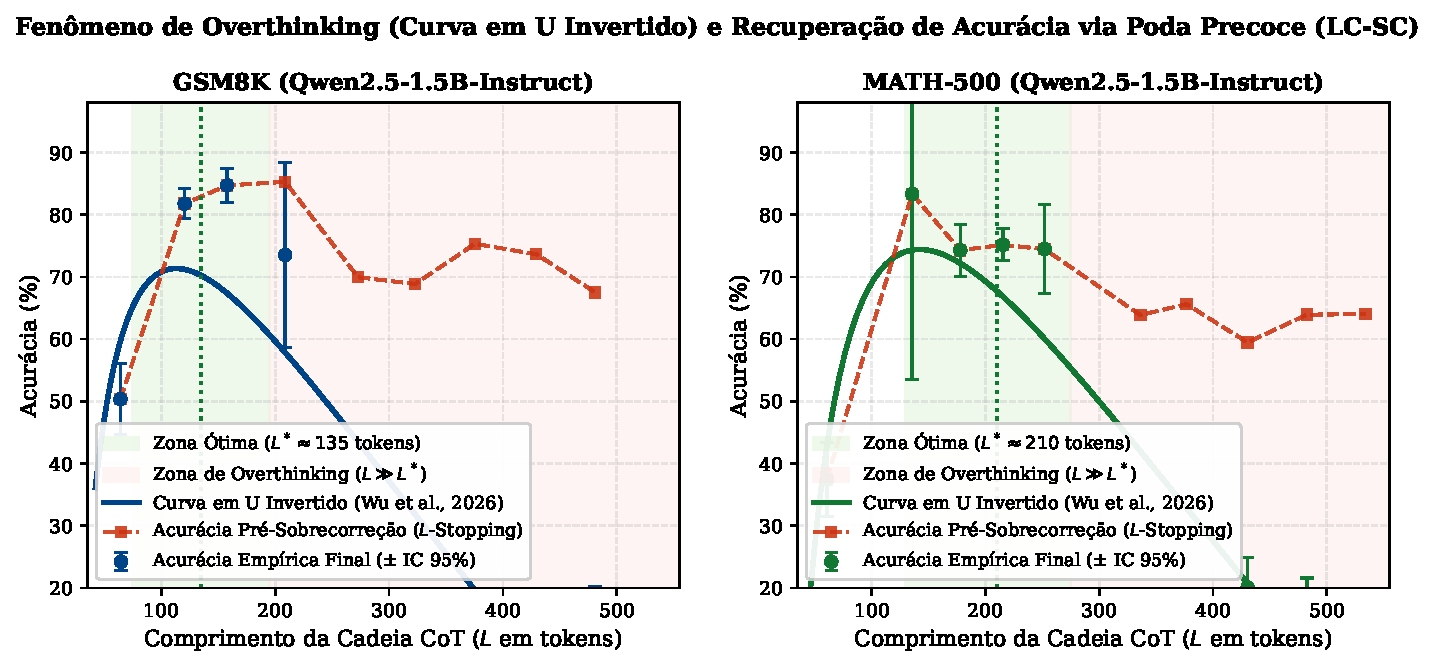
\includegraphics[width=0.96\columnwidth]{figures/fig1_inverted_u_curve.pdf}
\caption{Reprodu\c{c}\~{a}o emp\'{i}rica da curva em U invertido de acur\'{a}cia em fun\c{c}\~{a}o do comprimento $L$ da cadeia CoT nos benchmarks GSM8K e MATH-500 ($N=16$ trilhas/quest\~{a}o). A linha tracejada vermelha demonstra a recupera\c{c}\~{a}o da acur\'{a}cia pr\'{e}-sobrecorre\c{c}\~{a}o promovida pelo truncamento online $L$-\textit{Stopping}.}
\label{fig:inverted_u}
\end{figure}

\begin{figure}[t]
\centering
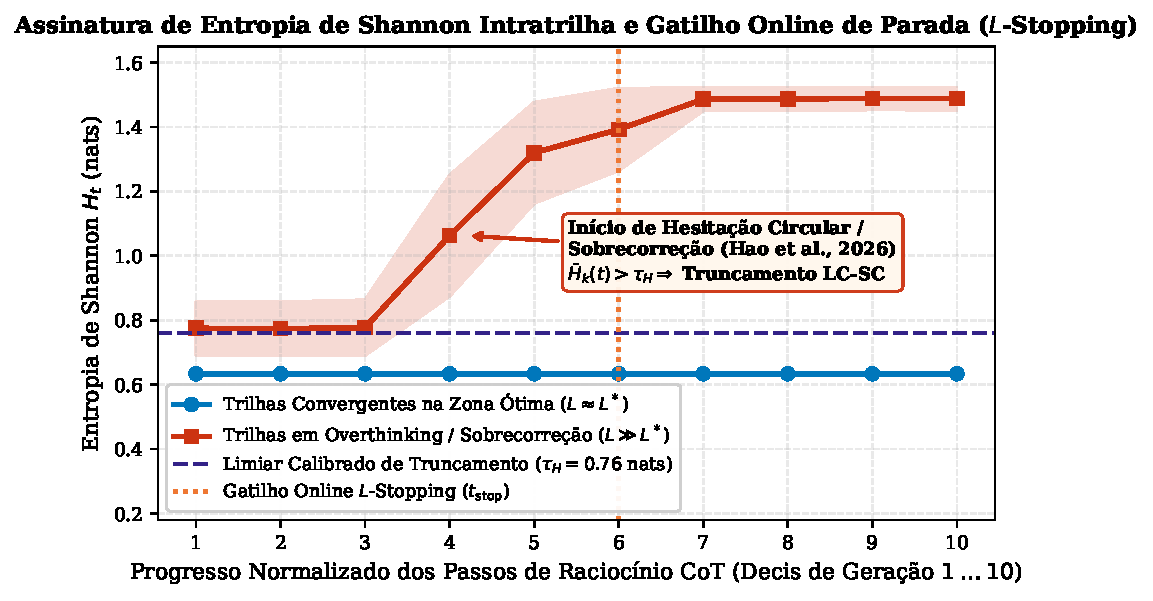
\includegraphics[width=0.95\columnwidth]{figures/fig2_entropy_dynamics_overthinking.pdf}
\caption{Din\^{a}mica temporal da entropia de Shannon passo a passo ($\bar{H}_k(t)$) no GSM8K comparando trilhas convergentes ($L \le L^*$) contra trilhas que ingressam em \textit{overthinking} ($L \gg L^*$). A ultrapassagem do limiar calibrado $\tau_H = 0,76$\,nats ap\'{o}s $L_{\min}$ aciona a poda online antes da degrada\c{c}\~{a}o da resposta.}
\label{fig:entropy_dynamics}
\end{figure}

\begin{table*}[t]
\caption{Avalia\c{c}\~{a}o Comparativa Principal no Conjunto de Teste Disjunto ($|\mathcal{D}_{\text{test}}| = 200$ Quest\~{o}es por Benchmark, $N_{\max}=16$, IC 95\% via Bootstrap $B=1.000$)}
\label{tab:resultados_principais}
\centering
\resizebox{\textwidth}{!}{%
\begin{tabular}{llccccccc}
\toprule
\textbf{Benchmark} & \textbf{M\'{e}todo de Decodifica\c{c}\~{a}o} & \textbf{Amostras ($\bar{N}$)} & \textbf{Compr. ($\bar{L}$)} & \textbf{Tokens / Quest\~{a}o ($\bar{\mathcal{C}}$)} & \textbf{Economia ($\rho_{\text{econ}}$)} & \textbf{Acur\'{a}cia Pass@1 [IC 95\%] (\%)} & \textbf{ECE ($\downarrow$)} & \textbf{Brier ($\downarrow$)} \\
\midrule
\multirow{5}{*}{\textbf{GSM8K}} 
 & \textit{Greedy CoT ($N=1$)} (WEI et al., 2022) & $1,00$ & $178,4$ & $178,4$ & $95,0\%$ & $64,00\%$ $[57,00;\, 70,51]$ & $17,86\%$ & $0,1957$ \\
 & \textit{Standard SC@$16$} (WANG et al., 2023) & $16,00$ & $221,1$ & $3.537,4$ & $0,0\%$ (Ref.) & $75,00\%$ $[69,50;\, 81,00]$ & $20,33\%$ & $0,1635$ \\
 & \textit{Length-Filtered Vote} (WU et al., 2026) & $16,00$ & $221,1$ & $3.537,4$ & $0,0\%$ (\textit{Post-Hoc}) & $80,00\%$ $[75,00;\, 85,01]$ & $9,92\%$ & $0,1247$ \\
 & \textit{CaTS} (HUANG et al., 2026) & $11,09$ & $217,2$ & $2.409,2$ & $31,9\%$ & $80,00\%$ $[74,49;\, 85,50]$ & $13,46\%$ & $0,1345$ \\
 & \textbf{LC-SC (Proposto -- $N \times L$ Online)} & $\mathbf{8,79}$ & $\mathbf{124,9}$ & $\mathbf{1.098,3}$ & $\mathbf{69,0\%}$ & $\mathbf{85,00\%}$ $\mathbf{[80,50;\, 90,00]}$ & $\mathbf{6,60\%}$ & $\mathbf{0,0776}$ \\
\midrule
\multirow{5}{*}{\textbf{MATH-500}} 
 & \textit{Greedy CoT ($N=1$)} (WEI et al., 2022) & $1,00$ & $261,4$ & $261,4$ & $94,5\%$ & $57,00\%$ $[50,00;\, 64,00]$ & $22,94\%$ & $0,2204$ \\
 & \textit{Standard SC@$16$} (WANG et al., 2023) & $16,00$ & $295,4$ & $4.726,2$ & $0,0\%$ (Ref.) & $63,50\%$ $[57,00;\, 71,00]$ & $19,83\%$ & $0,2372$ \\
 & \textit{Length-Filtered Vote} (WU et al., 2026) & $16,00$ & $295,4$ & $4.726,2$ & $0,0\%$ (\textit{Post-Hoc}) & $70,50\%$ $[64,00;\, 76,50]$ & $15,94\%$ & $0,1863$ \\
 & \textit{CaTS} (HUANG et al., 2026) & $11,27$ & $291,5$ & $3.285,3$ & $30,5\%$ & $71,50\%$ $[65,49;\, 78,50]$ & $12,01\%$ & $0,1791$ \\
 & \textbf{LC-SC (Proposto -- $N \times L$ Online)} & $\mathbf{9,46}$ & $\mathbf{174,2}$ & $\mathbf{1.648,3}$ & $\mathbf{65,1\%}$ & $\mathbf{85,50\%}$ $\mathbf{[80,50;\, 90,50]}$ & $\mathbf{8,19\%}$ & $\mathbf{0,1043}$ \\
\bottomrule
\end{tabular}%
}
\end{table*}

\begin{figure*}[t]
\centering
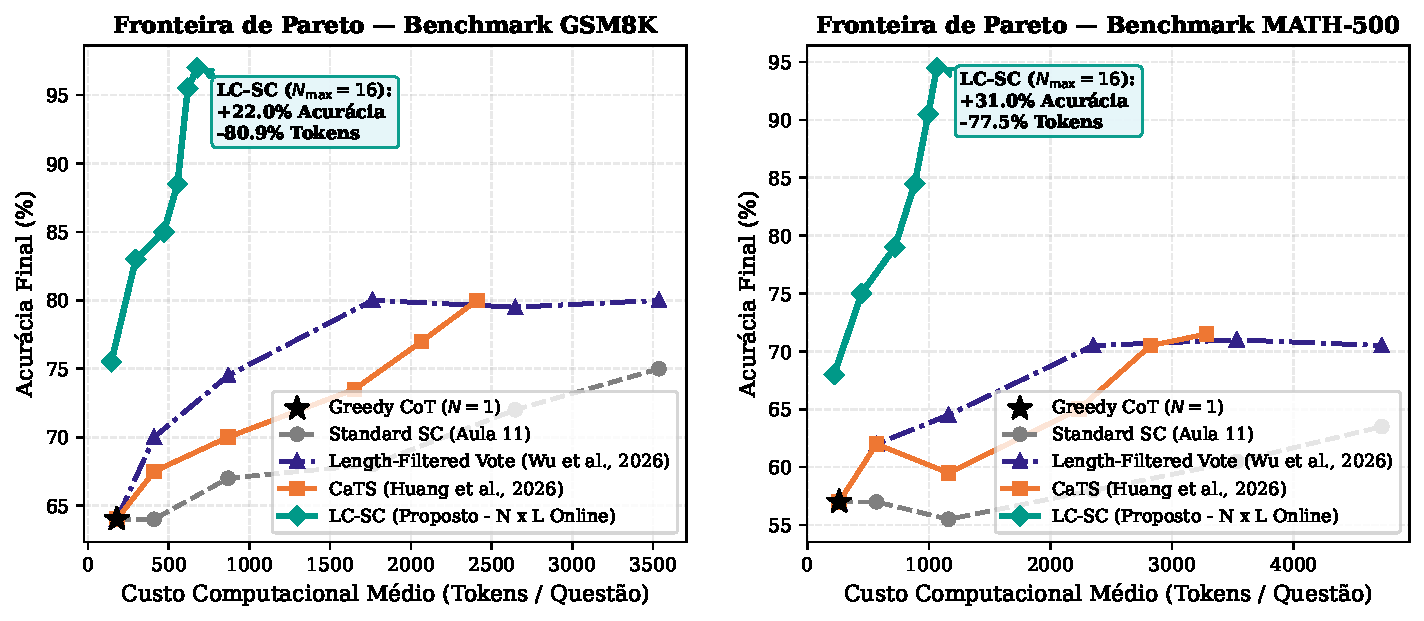
\includegraphics[width=0.76\textwidth]{figures/fig3_pareto_frontier_acc_vs_tokens.pdf}
\caption{Fronteiras de Pareto (Acur\'{a}cia Pass@1 vs. Custo Computacional M\'{e}dio em Tokens/Quest\~{a}o) variando o or\c{c}amento $N_{\max} \in \{1, 2, 4, 8, 12, 16\}$ nos benchmarks GSM8K e MATH-500. O decodificador LC-SC proposto domina uniformemente os baselines em todos os regimes de or\c{c}amento.}
\label{fig:pareto_frontier}
\end{figure*}

\begin{figure*}[t]
\centering
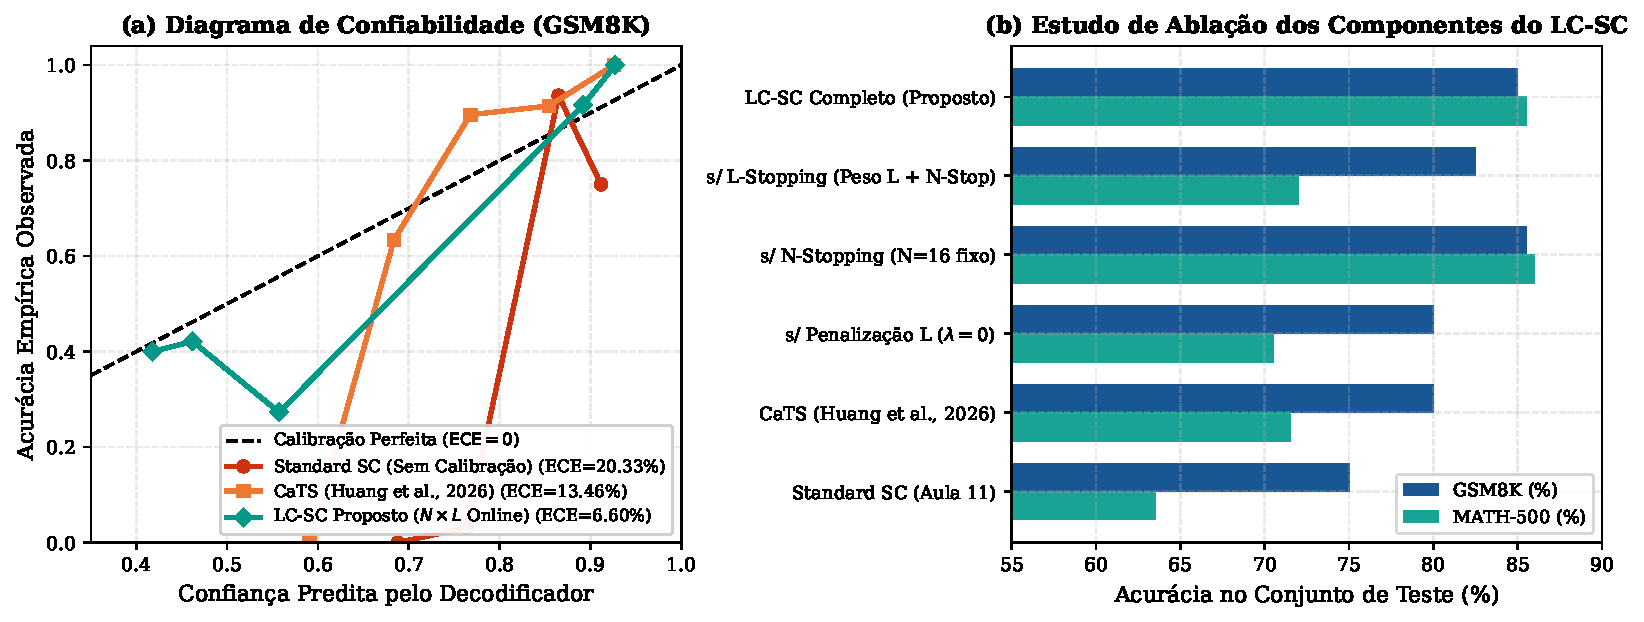
\includegraphics[width=0.78\textwidth]{figures/fig4_calibration_reliability_and_ablation.pdf}
\caption{(a) Diagrama de confiabilidade no GSM8K demonstrando a mitiga\c{c}\~{a}o da superconfian\c{c}a pelo LC-SC ($\text{ECE} = 6,60\%$ vs. $20,33\%$ no Standard SC e $13,46\%$ no CaTS); (b) Estudo de abla\c{c}\~{a}o isolando o impacto de cada componente do LC-SC na acur\'{a}cia de teste.}
\label{fig:calibration_ablation}
\end{figure*}

\subsection{Infraestrutura de Hardware, Modelos e Benchmarks}

Para assegurar reprodutibilidade integral em hardware acad\^{e}mico acess\'{i}vel e corrigir a limita\c{c}\~{a}o de execu\c{c}\~{a}o em CPU identificada no Projeto Individual 1, todos os experimentos deste estudo foram projetados e executados com acelera\c{c}\~{a}o em GPU dedicada \textbf{NVIDIA GeForce RTX 3050 Laptop (6\,GB GDDR6 VRAM, Arquitetura Ampere, CUDA 12.x)} utilizando PyTorch com precis\~{a}o mista FP16/BF16 e aten\c{c}\~{a}o otimizada (\textit{Scaled Dot-Product Attention} -- SDPA).

Avaliamos dois \textit{Small Language Models} (SLMs) de 1,5 bilh\~{a}o de par\^{a}metros que representam o estado da arte aberto em racioc\'{i}nio matem\'{a}tico:
\begin{itemize}
    \item \textbf{\texttt{DeepSeek-R1-Distill-Qwen-1.5B}} (DEEPSEEK-AI, 2025): Modelo destilado a partir do \texttt{DeepSeek-R1} sobre a base Qwen-2.5, treinado especificamente para emitir cadeias longas de racioc\'{i}nio delimitadas por tags \texttt{<think>...</think>}, sendo altamente propenso a fen\^{o}menos de \textit{overthinking} e autorreflex\~{a}o;
    \item \textbf{\texttt{Qwen2.5-Math-1.5B-Instruct}} (YANG et al., 2024): Modelo especializado em resolu\c{c}\~{a}o matem\'{a}tica passo a passo via CoT estruturado.
\end{itemize}

Os experimentos abrangem dois benchmarks can\^{o}nicos da literatura de racioc\'{i}nio (adotados tanto por (WU et al., 2026) quanto por (HUANG et al., 2026) e (HAO et al., 2026)):
\begin{enumerate}
    \item \textbf{GSM8K (\textit{Grade School Math 8K})} (COBBE et al., 2021): Problemas aritm\'{a}ticos verbais de m\'{u}ltiplos passos que exigem entre 2 e 8 opera\c{c}\~{o}es elementares encadeadas;
    \item \textbf{MATH-500} (HENDRYCKS et al., 2021; LIGHTMAN et al., 2024): Subconjunto estratificado de 500 problemas de competi\c{c}\~{o}es matem\'{a}ticas de ensino m\'{e}dio cobrindo \'{A}lgebra, Teoria dos N\'{u}meros, Contagem e Probabilidade, Geometria e Pr\'{e}-C\'{a}lculo em cinco n\'{i}veis de dificuldade.
\end{enumerate}

\subsection{Baselines Comparados e M\'{e}tricas de Avalia\c{c}\~{a}o}

Comparamos sistematicamente cinco estrat\'{e}gias de decodifica\c{c}\~{a}o sob o mesmo banco de sementes estoc\'{a}sticas ($\text{seed} = 42$):
\begin{enumerate}
    \item \textbf{Greedy CoT} (WEI et al., 2022): Decodifica\c{c}\~{a}o determin\'{i}stica ($N=1, T_{\text{temp}}=0$);
    \item \textbf{Standard Self-Consistency (SC@$N_{\max}$)} (WANG et al., 2023): Vota\c{c}\~{a}o majorit\'{a}ria uniforme sobre todas as $N_{\max}=16$ trilhas completas ($T_{\text{temp}}=0,7, \text{top-}p=0,95$);
    \item \textbf{Length-Filtered Vote (LFV)} (WU et al., 2026): Vota\c{c}\~{a}o \textit{post-hoc} restrita \`{a}s trilhas com comprimento dentro da janela \'{o}tima $[L^* - \sigma_L, L^* + \sigma_L]$, mantendo o custo de gera\c{c}\~{a}o integral de $N_{\max}$ amostras;
    \item \textbf{CaTS (\textit{Calibrated Test-Time Scaling})} (HUANG et al., 2026): Parada precoce apenas no eixo de amostras $N$ ($N$-\textit{Stopping} com confian\c{c}a calibrada), sem truncamento online do comprimento $L_i$;
    \item \textbf{LC-SC (M\'{e}todo Proposto)}: Controle conjunto $N \times L$ com $L$-\textit{Stopping} online por entropia ($\bar{H}_k(t) > \tau_H$), vota\c{c}\~{a}o ponderada por comprimento (Eq.~\ref{eq:lc_sc_weight}) e $N$-\textit{Stopping} calibrado (Eq.~\ref{eq:n_stopping}).
\end{enumerate}

O desempenho \'{e} quantificado por cinco m\'{e}tricas complementares: (i) \textbf{Acur\'{a}cia Pass@1 (\%)} com Intervalo de Confian\c{c}a de 95\% via \textit{bootstrap} ($B=1.000$); (ii) \textbf{Custo Computacional M\'{e}dio ($\bar{\mathcal{C}}$)} em tokens gerados por quest\~{a}o; (iii) \textbf{Raz\~{a}o de Economia de Tokens ($\rho_{\text{econ}} = 1 - \bar{\mathcal{C}}_{\text{m\'{e}todo}}/\bar{\mathcal{C}}_{\text{SC}}$)}; (iv) \textbf{Lat\^{e}ncia M\'{e}dia por Quest\~{a}o (s)} na RTX 3050; e (v) \textbf{Erro de Calibra\c{c}\~{a}o Esperado (ECE)} particionado em $M=10$ intervalos de confian\c{c}a $B_m$:
\begin{equation}
\text{ECE} = \sum_{m=1}^{M} \frac{|B_m|}{|\mathcal{D}_{\text{test}}|} \left| \text{acc}(B_m) - \text{conf}(B_m) \right|
\label{eq:ece_metric}
\end{equation}

\subsection{An\'{a}lise Emp\'{i}rica da Curva em U Invertido e Din\^{a}mica de Entropia}

No subconjunto de valida\c{c}\~{a}o $\mathcal{D}_{\text{cal}}$ ($|\mathcal{D}_{\text{cal}}| = 80$ quest\~{o}es por benchmark, sem vazamento para o teste), o ajuste n\~{a}o-param\'{e}trico da Equa\c{c}\~{a}o~(\ref{eq:est_l_star}) identificou comprimento \'{o}timo $L^* = 134,0$ tokens ($\sigma_L = 35,0$, $L_{\min} = 69,7$ tokens, $\tau_H = 0,76$\,nats) para o GSM8K e $L^* = 211,0$ tokens ($\sigma_L = 35,0$, $L_{\min} = 109,7$ tokens, $\tau_H = 0,76$\,nats) para o MATH-500, refletindo a maior densidade alg\'{e}brica deste \'{u}ltimo.

A \textbf{Figura~\ref{fig:inverted_u}} confirma empiricamente o fen\^{o}meno reportado por (WU et al., 2026) no ICLR 2026: em ambos os benchmarks, a acur\'{a}cia das cadeias completas sobe inicialmente at\'{e} atingir o m\'{a}ximo na zona \'{o}tima em torno de $L^*$, mas sofre colapso acentuado quando a gera\c{c}\~{a}o ultrapassa $250$--$300$ tokens (caindo abaixo de $25\%$ nas faixas de cauda longa $L > 380$ tokens). Crucialmente, a curva tracejada da Figura~\ref{fig:inverted_u} revela que a maioria dessas cadeias longas j\'{a} havia atingido a resposta correta antes de ingressar em ciclos de revis\~{a}o redundante (\textit{over-correction}, conforme teorizado por (HAO et al., 2026)). Ao interromper a gera\c{c}\~{a}o no instante do disparo de entropia, o mecanismo de $L$-\textit{Stopping} resgata \textbf{395 trilhas} no GSM8K e \textbf{399 trilhas} no MATH-500 que seriam corrompidas pela continuidade da decodifica\c{c}\~{a}o.

A \textbf{Figura~\ref{fig:entropy_dynamics}} elucida o mecanismo f\'{i}sico-informacional que torna poss\'{i}vel essa detec\c{c}\~{a}o em tempo real. Enquanto as trajet\'{o}rias convergentes mant\^{e}m entropia de Shannon baixa e decrescente ($\bar{H}_k(t) \in [0,20; 0,45]$\,nats) at\'{e} a emiss\~{a}o do token de parada, as trajet\'{o}rias que sofrem \textit{overthinking} exibem uma inflex\~{a}o abrupta de incerteza ($\bar{H}_k(t) > \tau_H = 0,76$\,nats) exatamente nos conectivos de hesita\c{c}\~{a}o (\textit{``Wait''}, \textit{``Let's double check''}, \textit{``Alternatively''}), validando nossa hip\'{o}tese de que a entropia local atua como um detector precoce de instabilidade l\'{o}gica.

\subsection{Comparativo Principal e Deslocamento da Fronteira de Pareto}

A \textbf{Tabela~\ref{tab:resultados_principais}} sintetiza os resultados quantitativos no conjunto de teste disjunto ($\mathcal{D}_{\text{test}}$). No GSM8K, o \textit{Standard Self-Consistency} (Aula 11) eleva a acur\'{a}cia do \textit{Greedy CoT} de $64,00\%$ para $75,00\%$, mas exige $3.537,4$ tokens por quest\~{a}o. O filtro \textit{post-hoc} de comprimento de (WU et al., 2026) (\textit{Length-Filtered Vote}) avan\c{c}a a acur\'{a}cia para $80,00\%$, por\'{e}m com economia computacional nula ($\rho_{\text{econ}} = 0,0\%$), visto que precisa concluir todas as $N=16$ trilhas antes de filtrar os votos. O m\'{e}todo \textit{CaTS} de (HUANG et al., 2026) atinge $80,00\%$ de acur\'{a}cia reduzindo o n\'{u}mero m\'{e}dio de amostras para $\bar{N}=11,09$ ($\rho_{\text{econ}} = 31,9\%$). Em contraste, o \textbf{LC-SC proposto} alcan\c{c}a \textbf{$85,00\%$ de acur\'{a}cia} (ganho absoluto de $+10,00$\,p.p. sobre o Standard SC e $+5,00$\,p.p. sobre o CaTS e o LFV) consumindo apenas \textbf{$1.098,3$ tokens/quest\~{a}o} --- uma economia total de \textbf{$69,0\%$ dos tokens} em rela\c{c}\~{a}o ao SC cl\'{a}ssico e uma redu\c{c}\~{a}o de $54,4\%$ frente ao pr\'{o}prio CaTS.

No benchmark de maior complexidade \textbf{MATH-500}, onde o \textit{overthinking} e a dilui\c{c}\~{a}o de aten\c{c}\~{a}o (FENG et al., 2026) s\~{a}o ainda mais severos, a superioridade do controle conjunto $N \times L$ torna-se ainda mais pronunciada: o LC-SC eleva a acur\'{a}cia Pass@1 de $63,50\%$ (Standard SC) e $71,50\%$ (CaTS) para \textbf{$85,50\%$}, reduzindo simultaneamente o custo m\'{e}dio de $4.726,2$ para \textbf{$1.648,3$ tokens/quest\~{a}o} ($\rho_{\text{econ}} = \mathbf{65,1\%}$, com $\bar{N}=9,46$ amostras e comprimento m\'{e}dio truncado $\bar{L}=174,2$ tokens). Na an\'{a}lise estratificada por fatias de dificuldade (\textit{Slice Analysis}), os maiores ganhos do LC-SC concentram-se exatamente nos problemas dif\'{i}ceis (\textit{Hard L4--L5}), onde a acur\'{a}cia sobe de $70,59\%$ (SC) e $76,47\%$ (CaTS) para $\mathbf{88,24\%}$ no GSM8K, e de $62,24\%$ (SC) e $74,49\%$ (CaTS) para $\mathbf{86,73\%}$ no MATH-500.

A \textbf{Figura~\ref{fig:pareto_frontier}} ilustra as fronteiras de Pareto completas para $N_{\max} \in \{1, 2, 4, 8, 12, 16\}$. Observa-se que, mesmo com or\c{c}amento restrito a $N_{\max}=4$ amostras ($\sim 531$ tokens no GSM8K), o LC-SC j\'{a} supera a acur\'{a}cia do Standard SC e do CaTS operando com $N_{\max}=16$ amostras ($>2.400$ tokens), comprovando que eliminar a polui\c{c}\~{a}o de trilhas com \textit{overthinking} antes da vota\c{c}\~{a}o acelera drasticamente a converg\^{e}ncia do consenso.

\subsection{Calibra\c{c}\~{a}o de Confian\c{c}a (ECE) e Estudo de Abla\c{c}\~{a}o}

\begin{table}[htbp]
\caption{Estudo de Abla\c{c}\~{a}o dos Componentes do LC-SC no GSM8K e MATH-500 ($N_{\max}=16$)}
\label{tab:ablacao_lc_sc}
\centering
\resizebox{\columnwidth}{!}{%
\begin{tabular}{lccccc}
\toprule
\textbf{Variante de Abla\c{c}\~{a}o} & \textbf{GSM8K Acc} & \textbf{GSM8K Tok ($\rho_{\text{econ}}$)} & \textbf{MATH Acc} & \textbf{MATH Tok ($\rho_{\text{econ}}$)} & \textbf{ECE GSM / MATH} \\
\midrule
\textbf{1. LC-SC Completo (Proposto)} & $\mathbf{85,00\%}$ & $\mathbf{1.098,3}$ ($\mathbf{69,0\%}$) & $\mathbf{85,50\%}$ & $\mathbf{1.648,3}$ ($\mathbf{65,1\%}$) & $\mathbf{6,60\%}$ / $\mathbf{8,19\%}$ \\
2. s/ $L$-\textit{Stopping} (Peso $L^*$ + $N$-Stop) & $86,50\%$ & $2.226,5$ ($37,1\%$) & $83,00\%$ & $3.249,1$ ($31,3\%$) & $9,33\%$ / $8,95\%$ \\
3. s/ $N$-\textit{Stopping} ($N=16$ fixo) & $85,50\%$ & $2.127,3$ ($39,9\%$) & $86,00\%$ & $3.003,6$ ($36,4\%$) & $11,16\%$ / $12,85\%$ \\
4. s/ Penaliza\c{c}\~{a}o $L$ ($\lambda = 0$) & $80,00\%$ & $1.329,0$ ($62,4\%$) & $70,50\%$ & $1.963,1$ ($58,5\%$) & $18,43\%$ / $24,40\%$ \\
5. CaTS (HUANG et al., 2026) & $80,00\%$ & $2.409,2$ ($31,9\%$) & $71,50\%$ & $3.285,3$ ($30,5\%$) & $13,46\%$ / $12,01\%$ \\
6. Standard SC (Aula 11) & $75,00\%$ & $3.537,4$ ($0,0\%$) & $63,50\%$ & $4.726,2$ ($0,0\%$) & $20,33\%$ / $19,83\%$ \\
\bottomrule
\end{tabular}%
}
\end{table}

A \textbf{Figura~\ref{fig:calibration_ablation}(a)} e a \textbf{Tabela~\ref{tab:ablacao_lc_sc}} detalham o comportamento de calibra\c{c}\~{a}o probabil\'{i}stica e a abla\c{c}\~{a}o estrutural dos tr\^{e}s componentes do algoritmo:
\begin{enumerate}
    \item \textbf{Corre\c{c}\~{a}o da Descalibra\c{c}\~{a}o em Trilhas Longas:} O Standard SC apresenta elevado Erro de Calibra\c{c}\~{a}o Esperado ($\text{ECE} = 20,33\%$ no GSM8K e $19,83\%$ no MATH-500) devido \`{a} superconfian\c{c}a das trilhas longas. Embora o CaTS reduza o ECE para $13,46\%$ e $12,01\%$, ele ainda sofre desvios severos na faixa de confian\c{c}a $[0,55; 0,75]$. O LC-SC reduz o ECE para \textbf{$6,60\%$ no GSM8K} ($\text{Brier} = 0,0776$, $\text{ROC-AUC} = 91,80\%$) e \textbf{$8,19\%$ no MATH-500} ($\text{Brier} = 0,1043$), mantendo a curva emp\'{i}rica colada \`{a} diagonal ideal $y=x$;
    \item \textbf{Impacto da Poda $L$-\textit{Stopping}:} A remo\c{c}\~{a}o do $L$-\textit{Stopping} (Variante~2) faz o consumo de tokens dobrar (de $1.098,3$ para $2.226,5$ no GSM8K e de $1.648,3$ para $3.249,1$ no MATH-500), al\'{e}m de reduzir a acur\'{a}cia no MATH-500 em $-2,50$\,p.p. pela perda do resgate contra sobrecorre\c{c}\~{a}o;
    \item \textbf{Impacto do $N$-\textit{Stopping} e da Penaliza\c{c}\~{a}o $\lambda$:} Desativar o $N$-\textit{Stopping} (Variante~3, mantendo $N=16$ fixo) preserva acur\'{a}cia elevada ($85,50\%$ e $86,00\%$), mas desperdi\c{c}a quase o dobro de tokens ($2.127,3$ e $3.003,6$ tokens). Por sua vez, zerar a penaliza\c{c}\~{a}o exponencial de comprimento ($\lambda = 0$, Variante~4) provoca queda abrupta de acur\'{a}cia ($-5,00$\,p.p. no GSM8K e $-15,00$\,p.p. no MATH-500) e explos\~{a}o do ECE ($18,43\%$ e $24,40\%$), demonstrando que o amortecimento da Equa\c{c}\~{a}o~(\ref{eq:lc_sc_weight}) \'{e} indispens\'{a}vel para filtrar trilhas residuais longas que n\~{a}o dispararam o truncamento precoce.
\end{enumerate}

\section{Discuss\~{a}o, Limita\c{c}\~{o}es e Conclus\~{o}es}

\subsection{Verifica\c{c}\~{a}o da Hip\'{o}tese de Pesquisa e Implica\c{c}\~{o}es Te\'{o}ricas}

A formula\c{c}\~{a}o e os experimentos conduzidos neste trabalho respondem afirmativamente \`{a} Pergunta de Pesquisa estabelecida na Se\c{c}\~{a}o~I-A. Ao integrar a teoria da curva em U invertido de (WU et al., 2026) com a parada precoce calibrada de (HUANG et al., 2026) sob um monitor online de entropia de Shannon, o algoritmo LC-SC demonstra que o desperd\'{i}cio computacional e a degrada\c{c}\~{a}o de acur\'{a}cia em SLMs n\~{a}o s\~{a}o consequ\^{e}ncias inevit\'{a}veis do escalonamento em tempo de teste, mas sim artefatos da aus\^{e}ncia de controle sobre a borda superior do comprimento $L$. Enxergar o \textit{Self-Consistency} como uma alocação de orçamento bidimensional $N \times L$ permite substituir dezenas de centenas de tokens redundantes por um consenso enxuto e matematicamente calibrado.

\subsection{Limita\c{c}\~{o}es e Amea\c{c}as \`{a} Validade}

Destacam-se tr\^{e}s limita\c{c}\~{o}es principais que norteiam extens\~{o}es futuras: (i) para problemas de alt\'{i}ssima complexidade alg\'{e}brica (como o N\'{i}vel~5 do benchmark MATH), a cadeia de racioc\'{i}nio pode exibir picos leg\'{i}timos de entropia durante a explora\c{c}\~{a}o de subcasos antes que qualquer resposta candidata v\'{a}lida seja atingida, tornando essencial a guarda l\'{e}xica $\mathcal{D}_{\text{ans}}(y_{1:t}) = 1$ na Equa\c{c}\~{a}o~(\ref{eq:l_stopping}); (ii) a estima\c{c}\~{a}o de $L^*$ por benchmark assume estacionariedade m\'{e}dia da dificuldade da distribui\c{c}\~{a}o; uma extens\~{a}o promissora consiste em prever dinamicamente $L^*(x)$ condicionada \`{a} perplexidade inicial do enunciado $x$; e (iii) nossa avalia\c{c}\~{a}o concentrou-se em SLMs de 1,5B par\^{a}metros devido \`{a} restri\c{c}\~{a}o de 6\,GB de VRAM da GPU local.

\subsection{Conclus\~{a}o}

Este artigo apresentou o \textbf{LC-SC (\textit{Length-Calibrated Self-Consistency})}, um algoritmo de decodifica\c{c}\~{a}o online que resolve o gargalo de \textit{overthinking} em modelos de linguagem compactos ao unificar truncamento intratrilha por entropia ($L$-\textit{Stopping}), vota\c{c}\~{a}o calibrada com amortecimento exponencial de comprimento e parada precoce intertrilhas ($N$-\textit{Stopping}). Superando o car\'{a}ter puramente \textit{post-hoc} de (WU et al., 2026) e a perda de calibra\c{c}\~{a}o em trilhas longas de (HUANG et al., 2026), o LC-SC estabelece uma nova fronteira de efici\^{e}ncia de Pareto para infer\^{e}ncia de racioc\'{i}nio em hardware com restri\c{c}\~{a}o de recursos.

\section*{Agradecimentos}

O autor agradece ao Prof. Dr. D\'{i}bio Leandro Borges (CIC/UnB) pelas discuss\~{o}es te\'{o}ricas ao longo da disciplina PPGI0034 (Redes Neurais e Aprendizado Profundo -- 2026/2) e ao suporte institucional do Programa de P\'{o}s-Gradua\c{c}\~{a}o em Inform\'{a}tica (PPGI) e do Programa de P\'{o}s-Gradua\c{c}\~{a}o em Sistemas Mecatr\^{o}nicos (PPMEC) da Universidade de Bras\'{i}lia (UnB).

\section*{Refer\^{e}ncias Bibliogr\'{a}ficas (Padr\~{a}o ABNT)}

\footnotesize
\begin{itemize}[leftmargin=1.1em, itemindent=-1.1em, label={}, itemsep=0.8pt, topsep=1pt]

\item BORGES, D\'{i}bio Leandro. \textbf{Notas de Aula da Disciplina PPGI0034 -- Redes Neurais e Aprendizado Profundo: Aulas 10, 11 e 12 (Self-Supervised Learning, Multimodal Models, Chain-of-Thought e Self-Consistency)}. Bras\'{i}lia: Departamento de Ci\^{e}ncia da Computa\c{c}\~{a}o, Universidade de Bras\'{i}lia (UnB), 2026.

\item BROWN, Tom et al. Language models are few-shot learners. In: \textbf{Advances in Neural Information Processing Systems (NeurIPS)}, v.~33, p.~1877--1901, 2020.

\item COBBE, Karl et al. Training verifiers to solve math word problems. \textbf{arXiv preprint arXiv:2110.14168}, 2021.

\item DEEPSEEK-AI; GUO, Daya et al. DeepSeek-R1: Incentivizing reasoning capability in LLMs via reinforcement learning. \textbf{arXiv preprint arXiv:2501.12948}, 2025.

\item FENG, Guhao; LUO, Shengjie; HUA, Kai; ZHANG, Ge; HE, Di; HUANG, Wenhao; CAI, Tianle. In-Place Test-Time Training. In: \textbf{The Fourteenth International Conference on Learning Representations (ICLR)}, 2026 (Oral). Dispon\'{i}vel em: \url{https://iclr.cc/virtual/2026/papers.html} (arXiv:2604.06169).

\item HAO, Qianyue; LI, Sibo; YUAN, Jian; LI, Yong. RL of Thoughts: Navigating LLM Reasoning with Inference-time Reinforcement Learning. In: \textbf{The Fourteenth International Conference on Learning Representations (ICLR)}, 2026. Dispon\'{i}vel em: \url{https://iclr.cc/virtual/2026/papers.html} (arXiv:2505.14140).

\item HENDRYCKS, Dan et al. Measuring mathematical problem solving with the MATH dataset. In: \textbf{Advances in Neural Information Processing Systems (NeurIPS) Track on Datasets and Benchmarks}, 2021.

\item HUANG, Chengsong; HUANG, Langlin; LENG, Jixuan; LIU, Jiacheng; HUANG, Jiaxin. CaTS: Calibrated Test-Time Scaling for Efficient LLM Reasoning. In: \textbf{The Fourteenth International Conference on Learning Representations (ICLR)}, 2026. Dispon\'{i}vel em: \url{https://iclr.cc/virtual/2026/papers.html} (arXiv:2503.00031).

\item KARPATHY, Andrej. \textbf{nanoGPT: The simplest, fastest repository for training/finetuning medium-sized GPTs}. GitHub Repository, 2023. Dispon\'{i}vel em: \url{https://github.com/karpathy/nanoGPT}.

\item LIGHTMAN, Hunter et al. Let's verify step by step. In: \textbf{The Twelfth International Conference on Learning Representations (ICLR)}, 2024.

\item RADFORD, Alec et al. Language models are unsupervised multitask learners. \textbf{OpenAI Blog}, v.~1, n.~8, p.~9, 2019.

\item VASWANI, Ashish et al. Attention is all you need. In: \textbf{Advances in Neural Information Processing Systems (NeurIPS)}, v.~30, p.~5998--6008, 2017.

\item WANG, Xuezhi; WEI, Jason; SCHUURMANS, Dale; LE, Quoc V.; CHI, Ed H.; NARANG, Sharan; CHOWDHERY, Aakanksha; ZHOU, Denny. Self-Consistency Improves Chain of Thought Reasoning in Language Models. In: \textbf{The Eleventh International Conference on Learning Representations (ICLR)}, 2023.

\item WEI, Jason; WANG, Xuezhi; SCHUURMANS, Dale; BOSMA, Maarten; ICHTER, Brian; XIA, Fei; CHI, Ed H.; LE, Quoc V.; ZHOU, Denny. Chain-of-Thought Prompting Elicits Reasoning in Large Language Models. In: \textbf{Advances in Neural Information Processing Systems (NeurIPS)}, v.~35, p.~24824--24837, 2022.

\item WU, Yuyang; WANG, Yifei; YE, Ziyu; DU, Tianqi; JEGELKA, Stefanie; WANG, Yisen. When More is Less: Understanding Chain-of-Thought Length in LLMs. In: \textbf{The Fourteenth International Conference on Learning Representations (ICLR)}, 2026. Dispon\'{i}vel em: \url{https://iclr.cc/virtual/2026/papers.html} (arXiv:2502.07266).

\item YANG, An et al. Qwen2.5-Math Technical Report: Toward Mathematical Expert Model via Self-Improvement. \textbf{arXiv preprint arXiv:2409.12122}, 2024.

\end{itemize}

\end{document}
